\documentclass[10pt]{article}
\usepackage[utf8]{inputenc}
\usepackage[T1]{fontenc}
\usepackage{graphicx}
\usepackage{amsmath}
\usepackage{geometry}
\usepackage{setspace}
\usepackage{booktabs}
\usepackage{float}
\usepackage{caption}
\usepackage{multirow}
\usepackage{hyperref}
\usepackage{longtable}
\usepackage{caption}

\captionsetup[figure]{labelformat=empty}
\captionsetup[table]{labelformat=empty}


\geometry{margin=1in, footskip=0.5in}
\onehalfspacing

\title{Supplementary Information:\\
Decadal Surface Water Dynamics in Bangladesh Using Sentinel-1 SAR (2015--2025)}
\author{}
\date{}

\begin{document}
\maketitle

% =========================
% Supplementary Figure S1 - Study Area
% =========================
% Note: Study area map is included in the main text (Figure 5).
% If journal requires separate figure files, export from main text.

% =========================
% Supplementary Figure S2 - Methodological Flowchart
% =========================
\begin{figure}[H]
    \centering
    
\includegraphics[width=1.0\textwidth]{figures/fig2_flowchart.pdf}
    \caption{\textbf{Supplementary Figure S1.} Methodological framework for decadal surface water monitoring in Bangladesh using Sentinel-1 SAR and seasonally adaptive thresholding.}
    \label{fig:s_flowchart}
\end{figure}

% =========================
% Supplementary Table S1 - Sentinel-1 Specs and Scene Counts
% =========================
\begin{table}[H]
\centering
\caption*{\textbf{Supplementary Table S1.} Sentinel-1 SAR data specifications and number of scenes used per year.}
\label{tab:s_specs}
\begin{tabular}{ll}
\toprule
\textbf{Parameter} & \textbf{Value} \\
\midrule
Satellite & Sentinel-1A/B \\
Product & GRD (Ground Range Detected) \\
Mode & IW (Interferometric Wide) \\
Polarization & VV \\
Spatial Resolution & 10 m \\
Temporal Coverage & January 2015 -- December 2025 \\
Temporal Resolution & 12 days (6 days with dual satellite) \\
Band & Sigma0 (dB) \\
Processing Level & Pre-processed (GEE) \\
\bottomrule
\end{tabular}
\end{table}

\begin{table}[H]
\centering
\caption*{\textbf{Supplementary Table S2.} Number of Sentinel-1 scenes used per year for Bangladesh.}
\begin{tabular}{lccccccccccc}
\toprule
\textbf{Year} & 2015 & 2016 & 2017 & 2018 & 2019 & 2020 & 2021 & 2022 & 2023 & 2024 & 2025 \\
\midrule
Scenes & 304 & 480 & 612 & 785 & 812 & 830 & 845 & 790 & 815 & 851 & 767 \\
\bottomrule
\end{tabular}
\end{table}

\begin{table}[H]
\centering
\caption{\textbf{Supplementary Table S3.} Monthly surface water area statistics (km$^{2}$) for Bangladesh (2015--2025). Values derived from GMM-based adaptive thresholds.}
\label{tab:s_monthly_water}
\begin{tabular}{lrrrr}
\toprule
\textbf{Month} & \textbf{Min} & \textbf{Max} & \textbf{Mean} & \textbf{Std.\ Dev.} \\
\midrule
January   & 13,290 & 16,744 & 15,332 & 931 \\
February  & 13,136 & 15,073 & 14,580 & 715 \\
March     & 13,049 & 15,352 & 14,534 & 811 \\
April     & 9,715  & 22,424 & 15,046 & 2,964 \\
May       & 13,740 & 24,806 & 17,749 & 4,084 \\
June      & 17,836 & 36,895 & 27,641 & 5,304 \\
July      & 30,442 & 48,577 & 37,504 & 5,915 \\
August    & 30,069 & 44,336 & 35,486 & 4,331 \\
September & 29,548 & 39,288 & 33,812 & 2,968 \\
October   & 24,374 & 34,373 & 29,511 & 3,062 \\
November  & 19,808 & 26,849 & 23,248 & 2,137 \\
December  & 16,432 & 21,069 & 18,652 & 1,340 \\
\bottomrule
\end{tabular}
\end{table}

% Items re-indexed below


% =========================
% Supplementary Table S2 - Monthly VV Thresholds
% =========================
\begin{table}[H]
\centering
\caption{\textbf{Supplementary Table S4.} Monthly VV backscatter thresholds (dB) derived from GMM analysis.}
\begin{tabular}{lclc}
\toprule
\textbf{Month} & \textbf{$\tau$ (dB)} & \textbf{Month} & \textbf{$\tau$ (dB)} \\
\midrule
January   & $-17.5$ & July      & $-13.8$ \\
February  & $-16.8$ & August    & $-13.8$ \\
March     & $-16.2$ & September & $-14.5$ \\
April     & $-15.5$ & October   & $-15.2$ \\
May       & $-14.8$ & November  & $-16.5$ \\
June      & $-14.2$ & December  & $-17.2$ \\
\bottomrule
\end{tabular}
\end{table}


% =========================
% Supplementary Figure S3 - Threshold Histograms
% =========================
\begin{figure}[H]
    \centering
    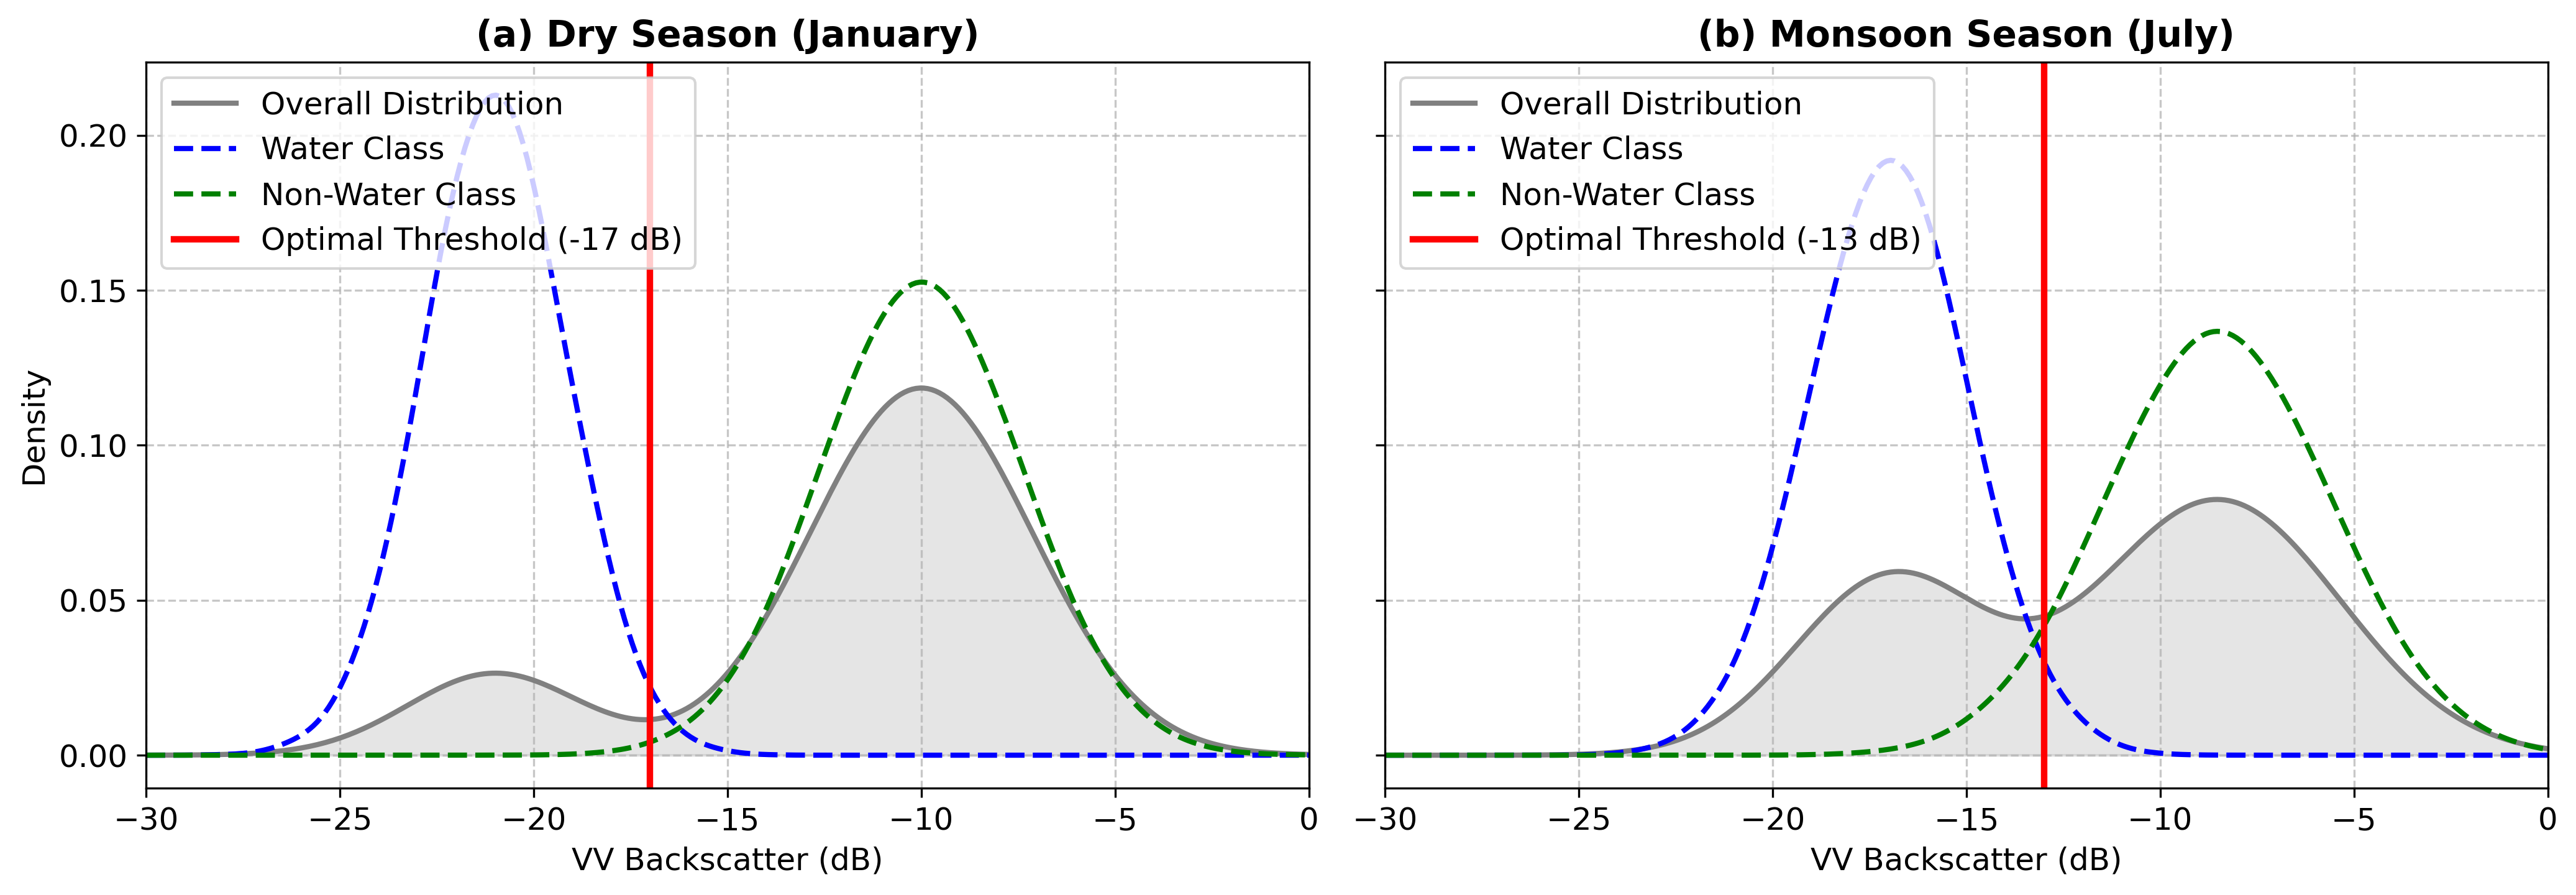
\includegraphics[width=1.0\textwidth]{figures/fig_threshold_histogram.png}
    \caption{\textbf{Supplementary Figure S2.} Representative bimodal distributions of Sentinel-1 VV backscatter for (a) the dry season (January) and (b) the monsoon season (July). Vertical lines indicate GMM-calibrated optimal thresholds.}
    \label{fig:s_threshold}
\end{figure}


% =========================
% Supplementary Table S3 - Water Persistence
% =========================
\begin{table}[H]
\centering
\caption{\textbf{Supplementary Table S5.} Water persistence classification for Bangladesh (averaged over 2015--2025).}
\begin{tabular}{lrr}
\toprule
\textbf{Persistence Class} & \textbf{Area (km$^{2}$)} & \textbf{\% of Bangladesh} \\
\midrule
Permanent ($F \geq 10$)         & 4,991.1 & 3.4 \\
Semi-permanent ($5 \leq F < 10$) & 11,471.1  & 7.8  \\
Ephemeral ($1 \leq F < 5$)      & 43,048.6 & 29.2 \\
No water ($F = 0$)              & 88,059.2 & 59.6 \\
\bottomrule
\end{tabular}
\end{table}


% =========================
% Supplementary Table S4 - Change Detection
% =========================
\begin{table}[H]
\centering
\caption{\textbf{Supplementary Table S6.} Inter-annual surface water change for July (2015 vs.\ 2025).}
\begin{tabular}{lrr}
\toprule
\textbf{Change Class} & \textbf{Area (km$^{2}$)} & \textbf{\% of Total Water} \\
\midrule
Gained & 6,304.7 & 21.5 \\
Stable & 15,270.9 & 52.0 \\
Lost   & 7,783.5  & 26.5 \\
\bottomrule
\end{tabular}
\end{table}


% =========================
% Supplementary Table S5 - Seasonal Extent
% =========================
\begin{table}[H]
\centering
\caption{\textbf{Supplementary Table S7.} Seasonal surface water extent (km$^{2}$) for Bangladesh (2015--2025, 11-year mean monthly average per season).}
\begin{tabular}{lrrr}
\toprule
\textbf{Season} & \textbf{Mean Area} & \textbf{Max Area} & \textbf{Min Area} \\
\midrule
Dry Winter (Dec--Feb)     & 15,927 & 21,069 & 13,136 \\
Pre-Monsoon (Mar--May)    & 15,715 & 24,806 & 9,715 \\
Monsoon (Jun--Sep)        & 33,611 & 48,577 & 17,836 \\
Post-Monsoon (Oct--Nov)   & 26,380 & 34,373 & 19,808 \\
\bottomrule
\end{tabular}
\end{table}


% =========================
% Supplementary Figure S4-S6 - Maps
% =========================
\begin{figure}[H]
    \centering
    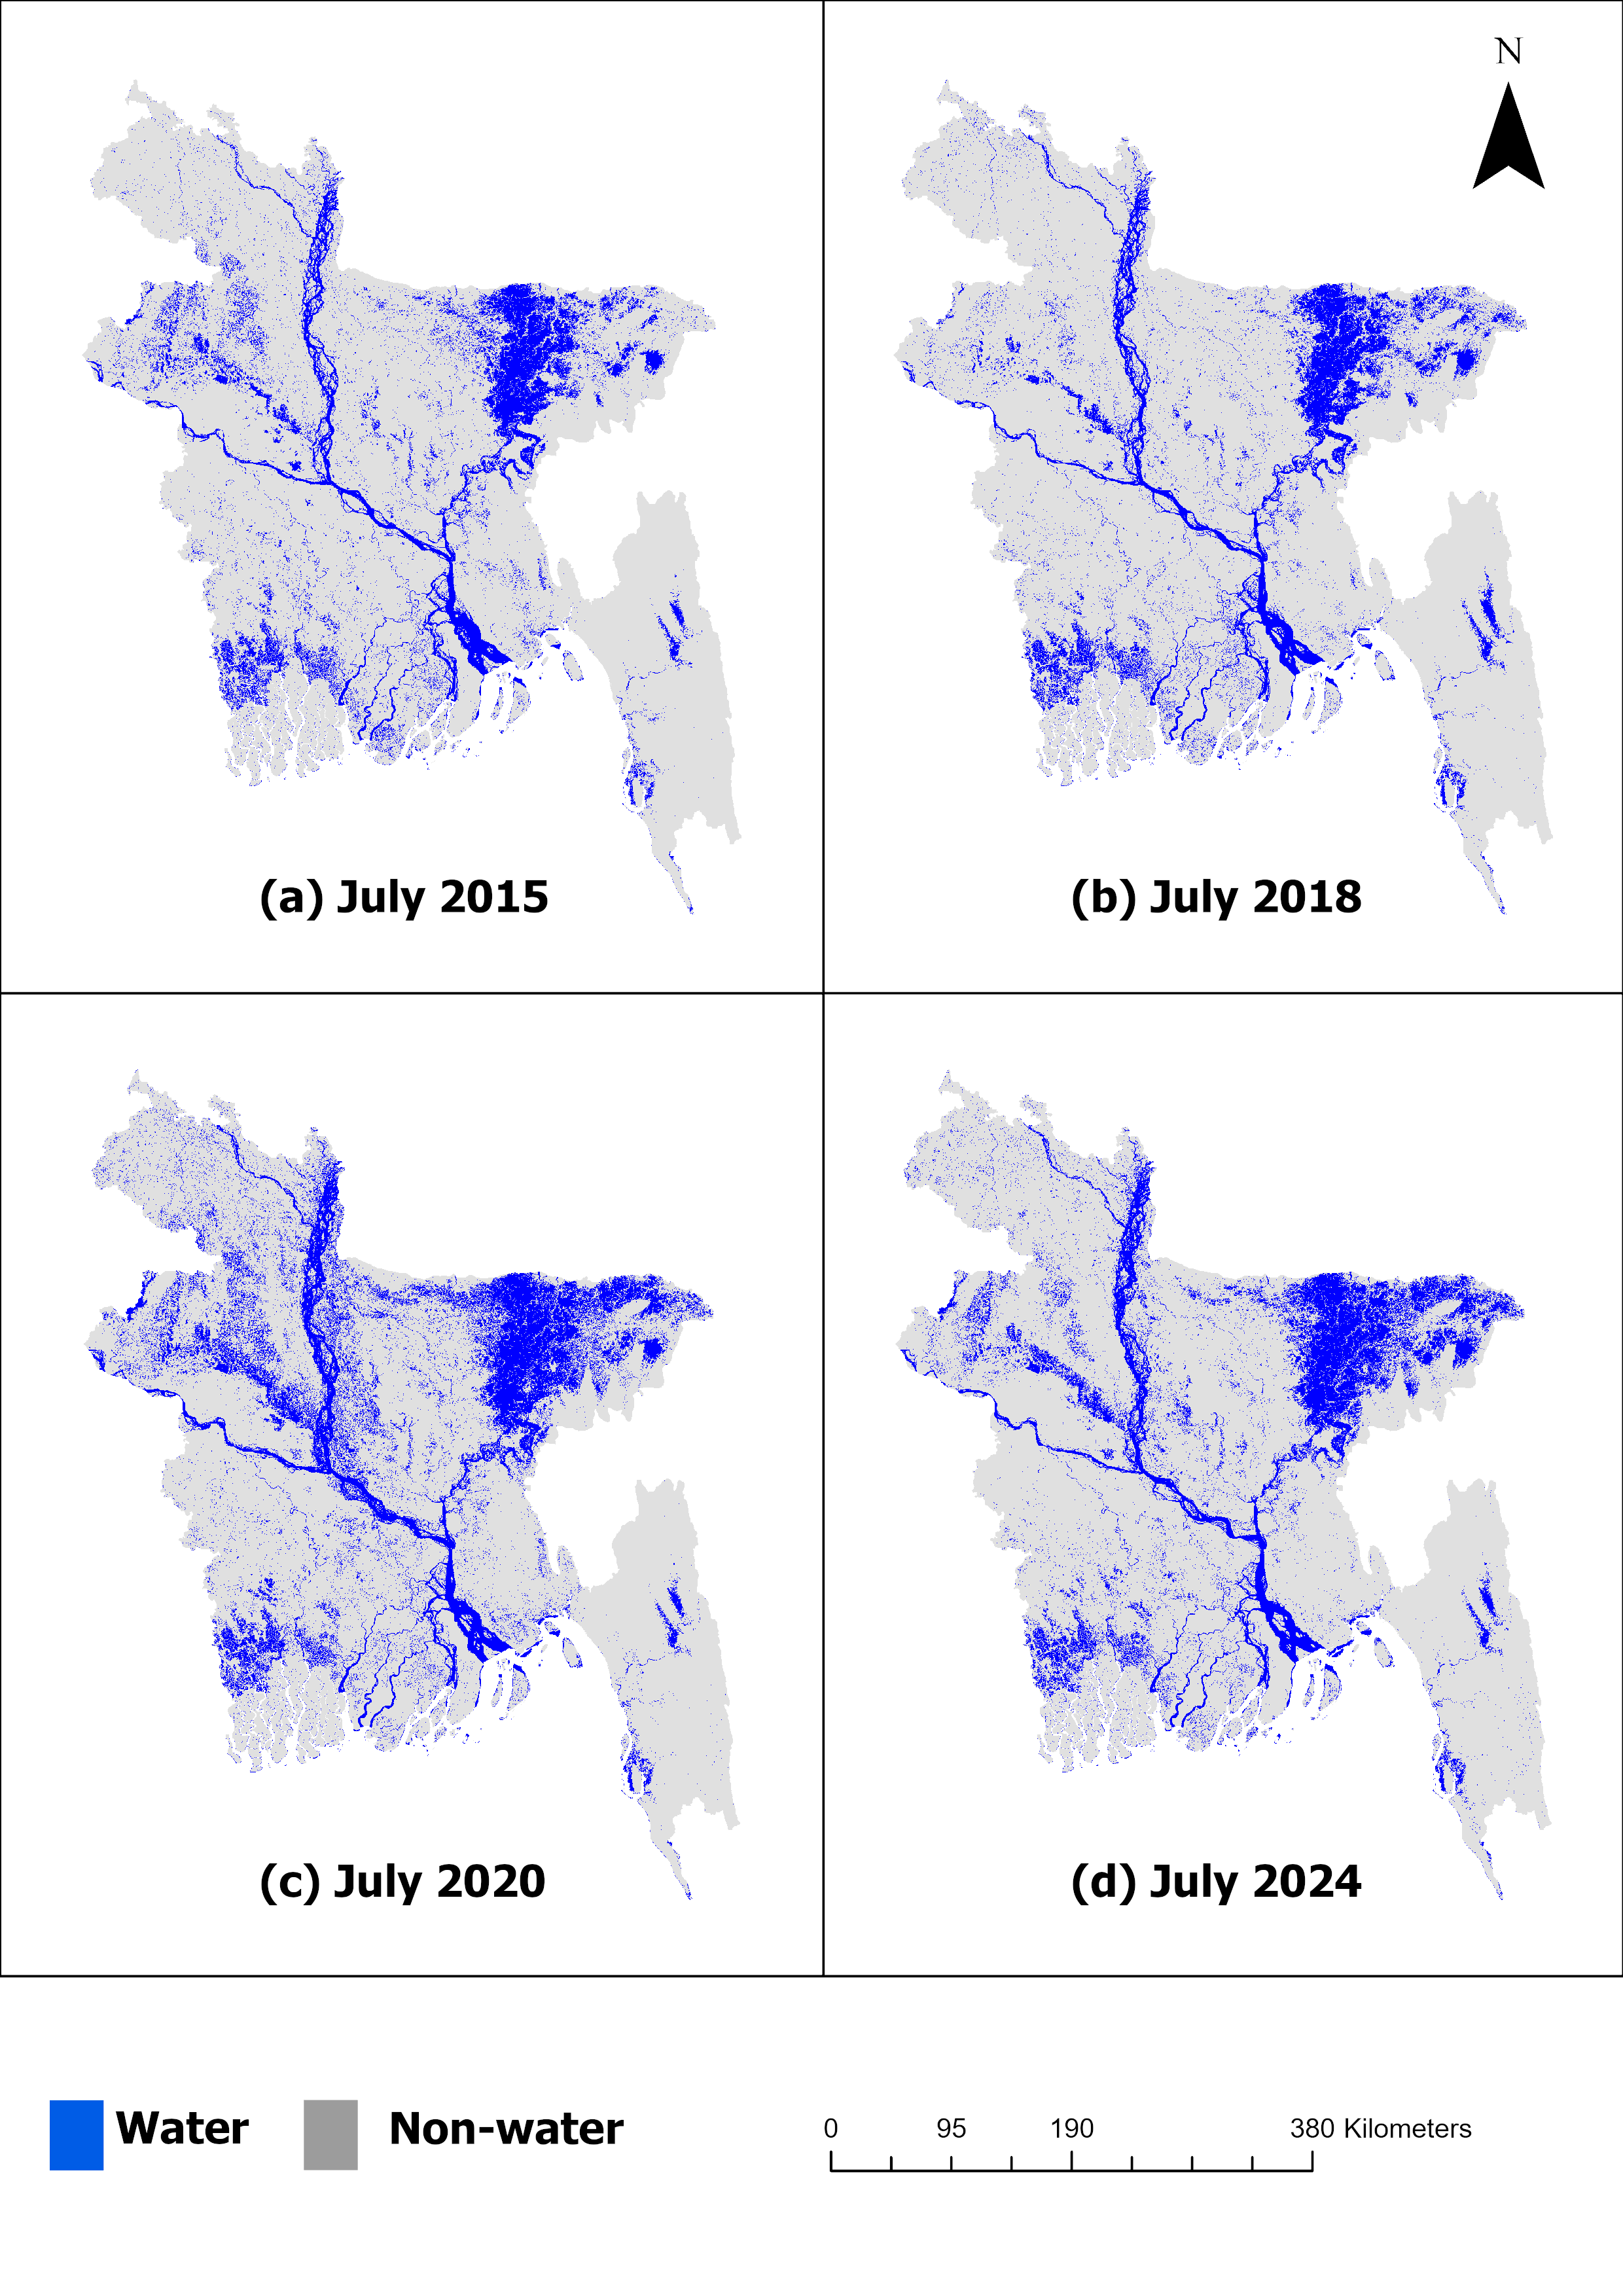
\includegraphics[width=0.9\textwidth]{figures/fig3_july_water_maps.png}
    \caption{\textbf{Supplementary Figure S3.} Spatiotemporal distribution of monthly surface water extent in Bangladesh for July across selected years (2015, 2018, 2020, 2024).}
    \label{fig:s_july_maps}
\end{figure}

\begin{figure}[H]
    \centering
    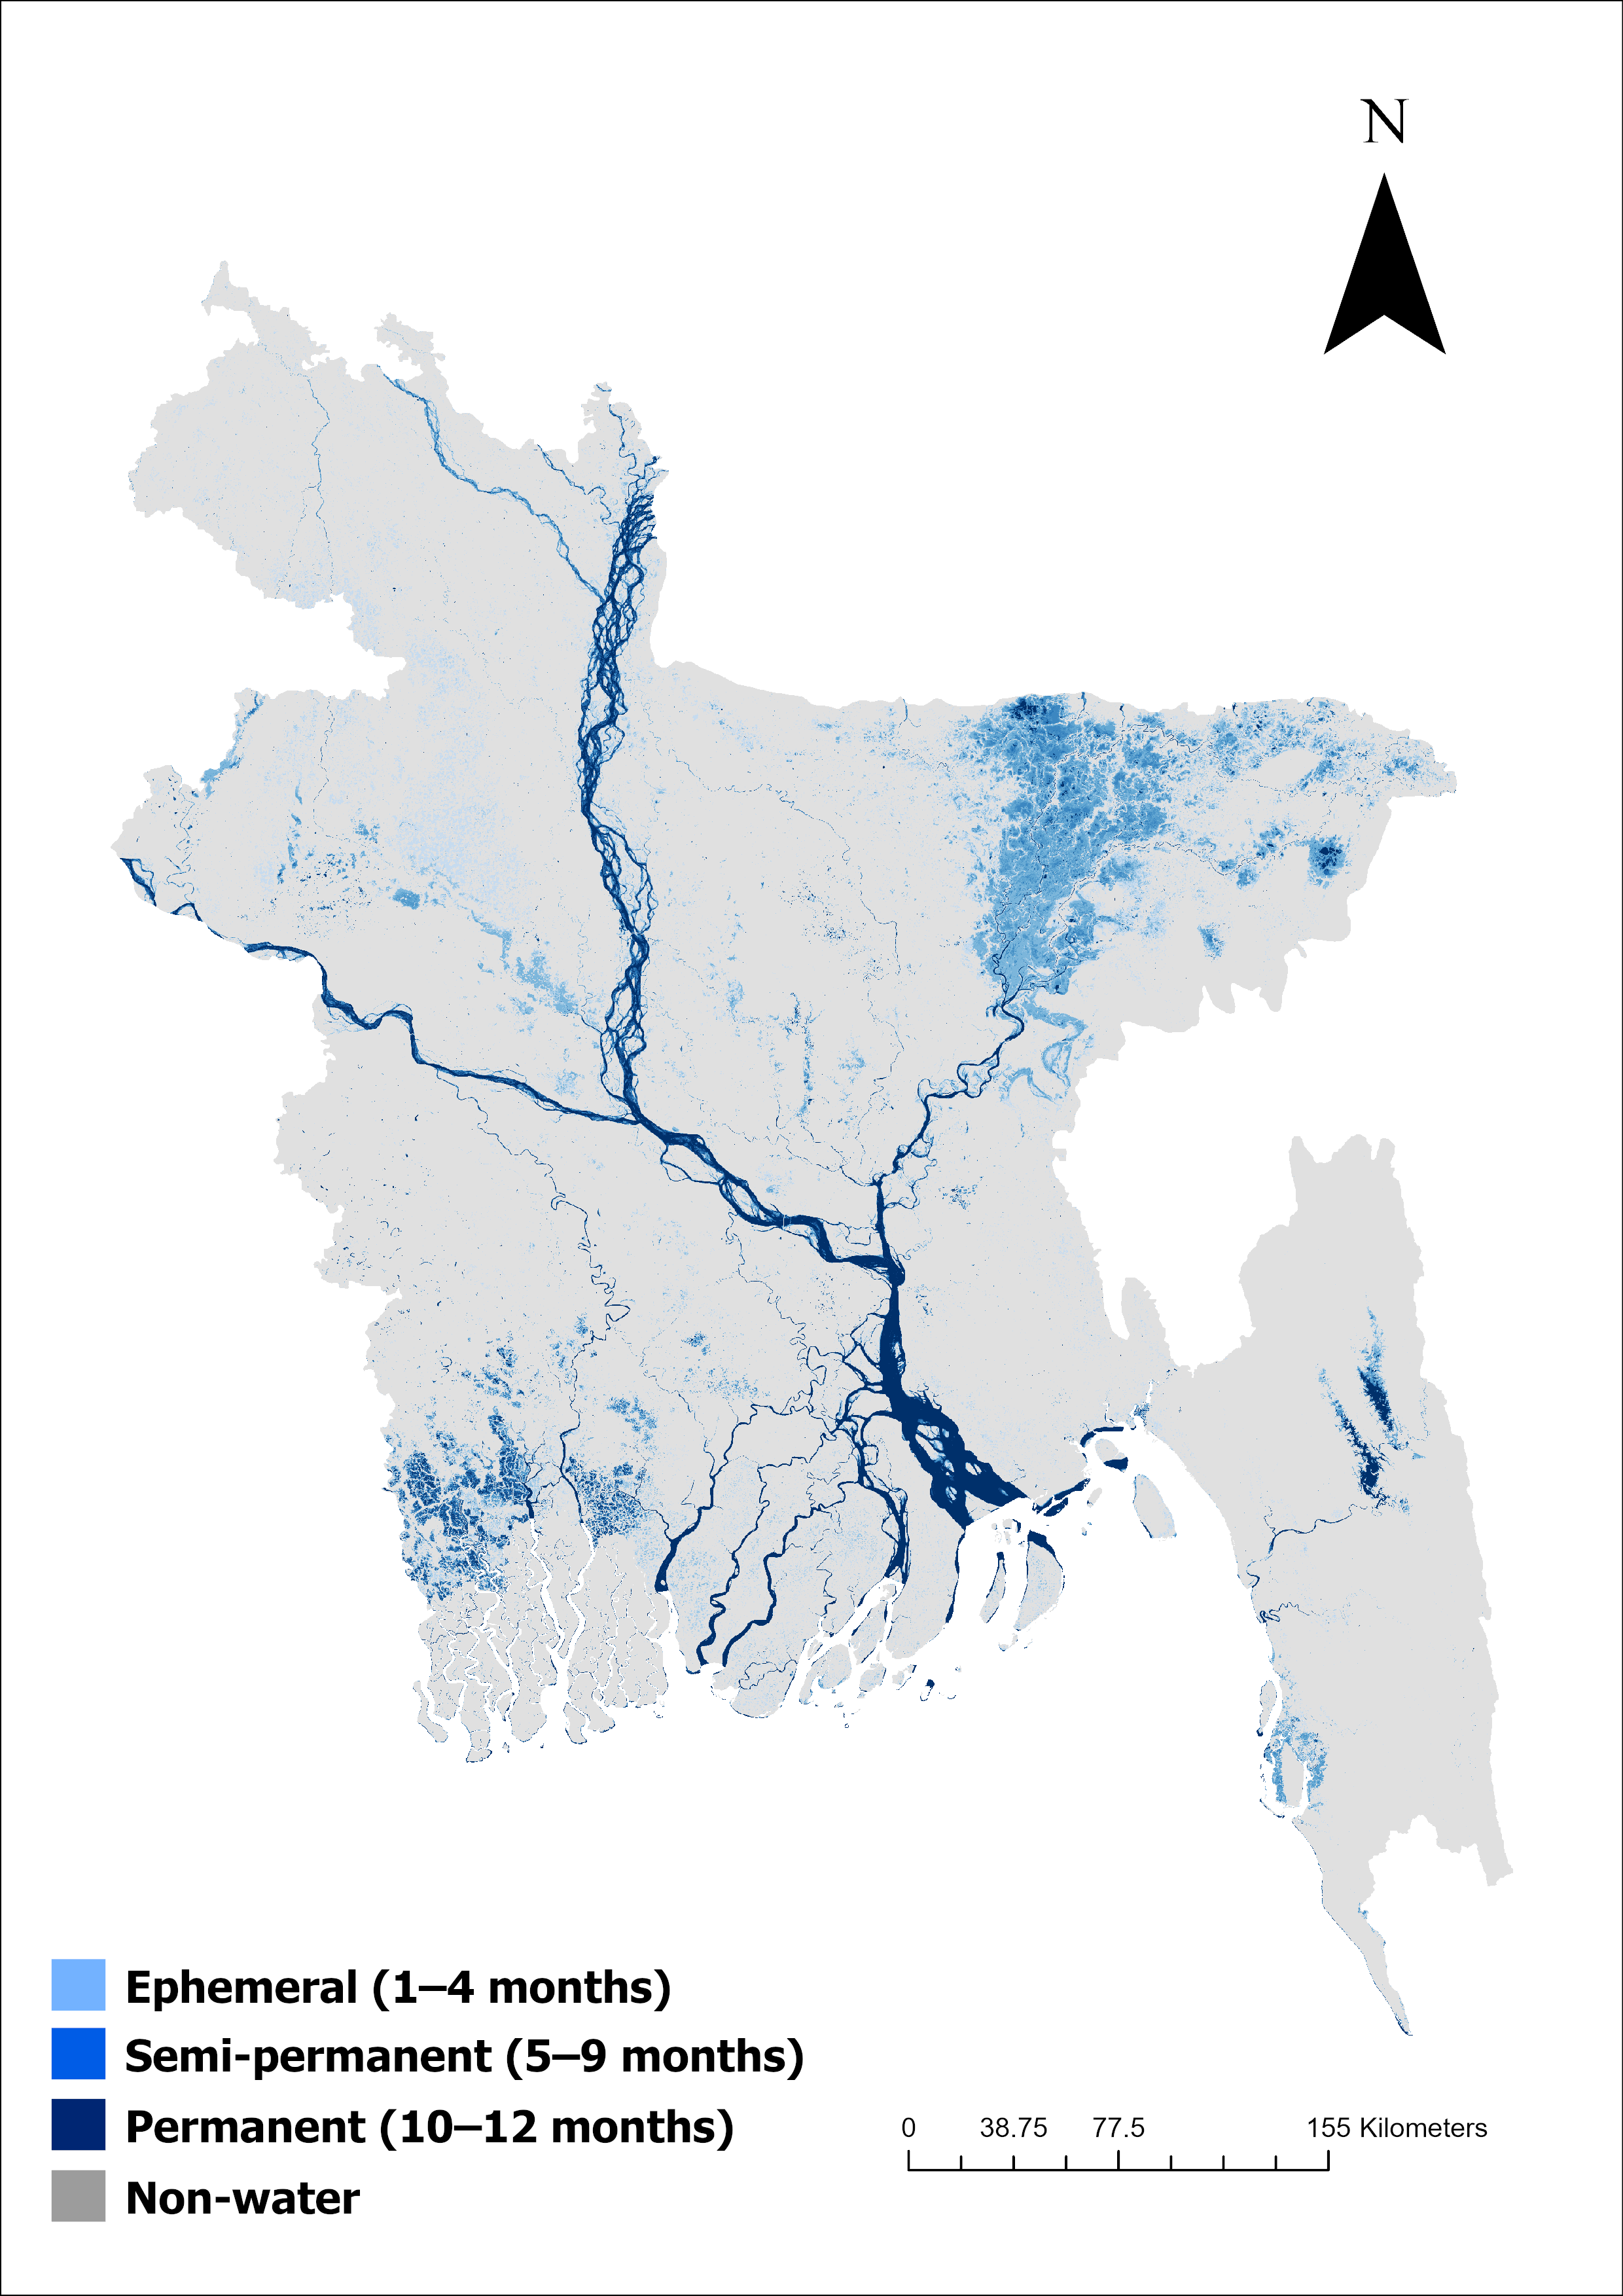
\includegraphics[width=0.85\textwidth]{figures/fig5_occurrence_2023.png}
    \caption{\textbf{Supplementary Figure S4.} Annual water occurrence frequency map for 2023.}
    \label{fig:s_occurrence}
\end{figure}

\begin{figure}[H]
    \centering
    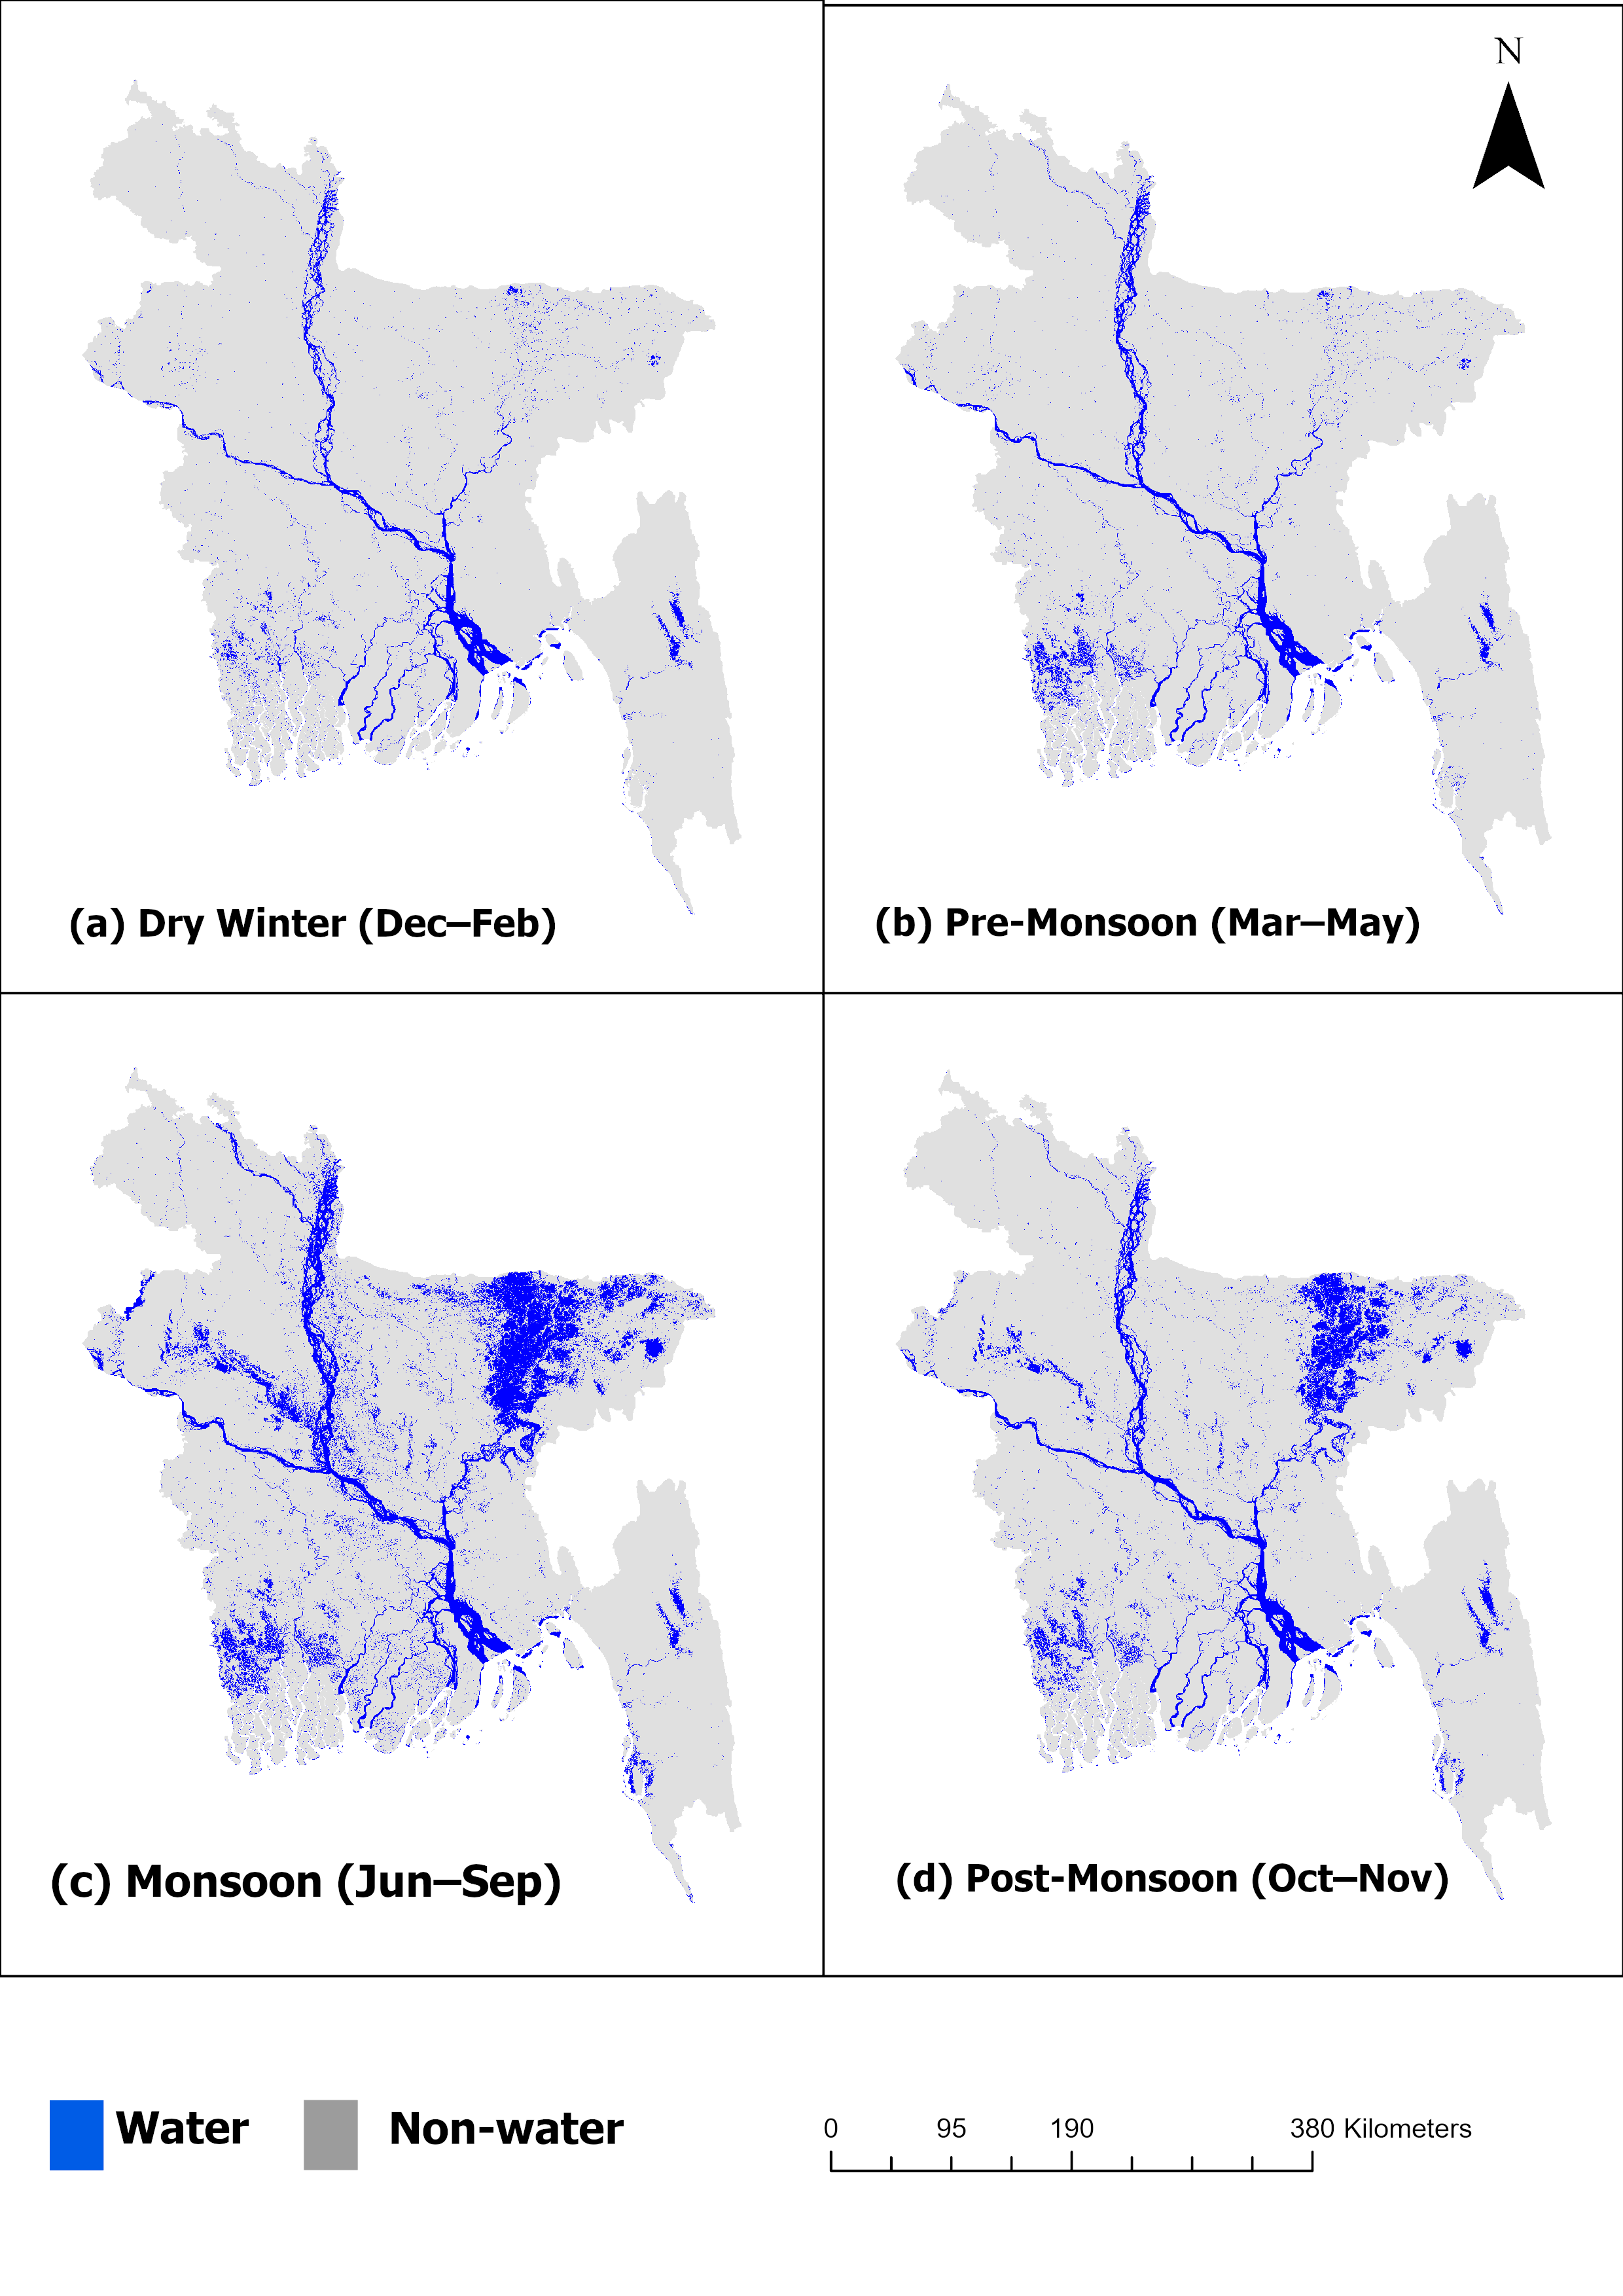
\includegraphics[width=0.9\textwidth]{figures/fig6_seasonal_maps.png}
    \caption{\textbf{Supplementary Figure S5.} Seasonal surface water distribution in Bangladesh for the four hydrological seasons.}
    \label{fig:s_seasonal}
\end{figure}

\begin{figure}[H]
    \centering
    
\includegraphics[width=0.9\textwidth]{figures/fig6_divisional_heatmap.png}
    \caption{\textbf{Supplementary Figure S6.} Divisional peak monsoon water extent heatmap (July, 2015--2025).}
    \label{fig:s_heatmap}
\end{figure}


% =========================
% Supplementary Figures S7-S8 - Additional Trend Plots
% =========================
\begin{figure}[H]
    \centering
    
\includegraphics[width=0.95\textwidth]{figures/fig7_annual_mean_trend.png}
    \caption{\textbf{Supplementary Figure S7.} Annual mean surface water area in Bangladesh (2015--2025) with linear regression trend.}
    \label{fig:s_annual_mean}
\end{figure}

\begin{figure}[H]
    \centering
    
\includegraphics[width=0.95\textwidth]{figures/fig9_top10_districts.png}
    \caption{\textbf{Supplementary Figure S8.} Top 10 most flood-prone districts in Bangladesh ranked by 11-year mean July surface water extent (2015--2025).}
    \label{fig:s_top10}
\end{figure}

\begin{figure}[H]
    \centering
    
\includegraphics[width=0.8\textwidth]{figures/fig8_monthly_boxplot.png}
    \caption{\textbf{Supplementary Figure S9.} Boxplot distribution of monthly surface water area across 11 years (2015--2025).}
    \label{fig:s_boxplot}
\end{figure}


% Figure moved to main text (Figure 6)


% =========================
% Supplementary Table S6 - Accuracy Detail
% =========================
\begin{table}[H]
\centering
\caption{\textbf{Supplementary Table S8.} Summary of accuracy metrics for the 4,310-point decadal baseline validation (2015--2025). OA = Overall Accuracy; PA = Producer's Accuracy; UA = User's Accuracy.}
\label{tab:s_accuracy}
\begin{tabular}{lr}
\toprule
\textbf{Metric} & \textbf{Value (\%)} \\
\midrule
Overall Accuracy (OA)        & 92.55\% \\
Kappa Coefficient ($\kappa$) & 0.8508  \\
Producer's Accuracy (PA)     & 96.78\% \\
User's Accuracy (UA)         & 87.81\% \\
F1 Score                     & 92.08\% \\
\bottomrule
\end{tabular}
\end{table}


% =========================
% Supplementary Figures S11-S12 - Validation Plots
% =========================
\begin{figure}[H]
    \centering
    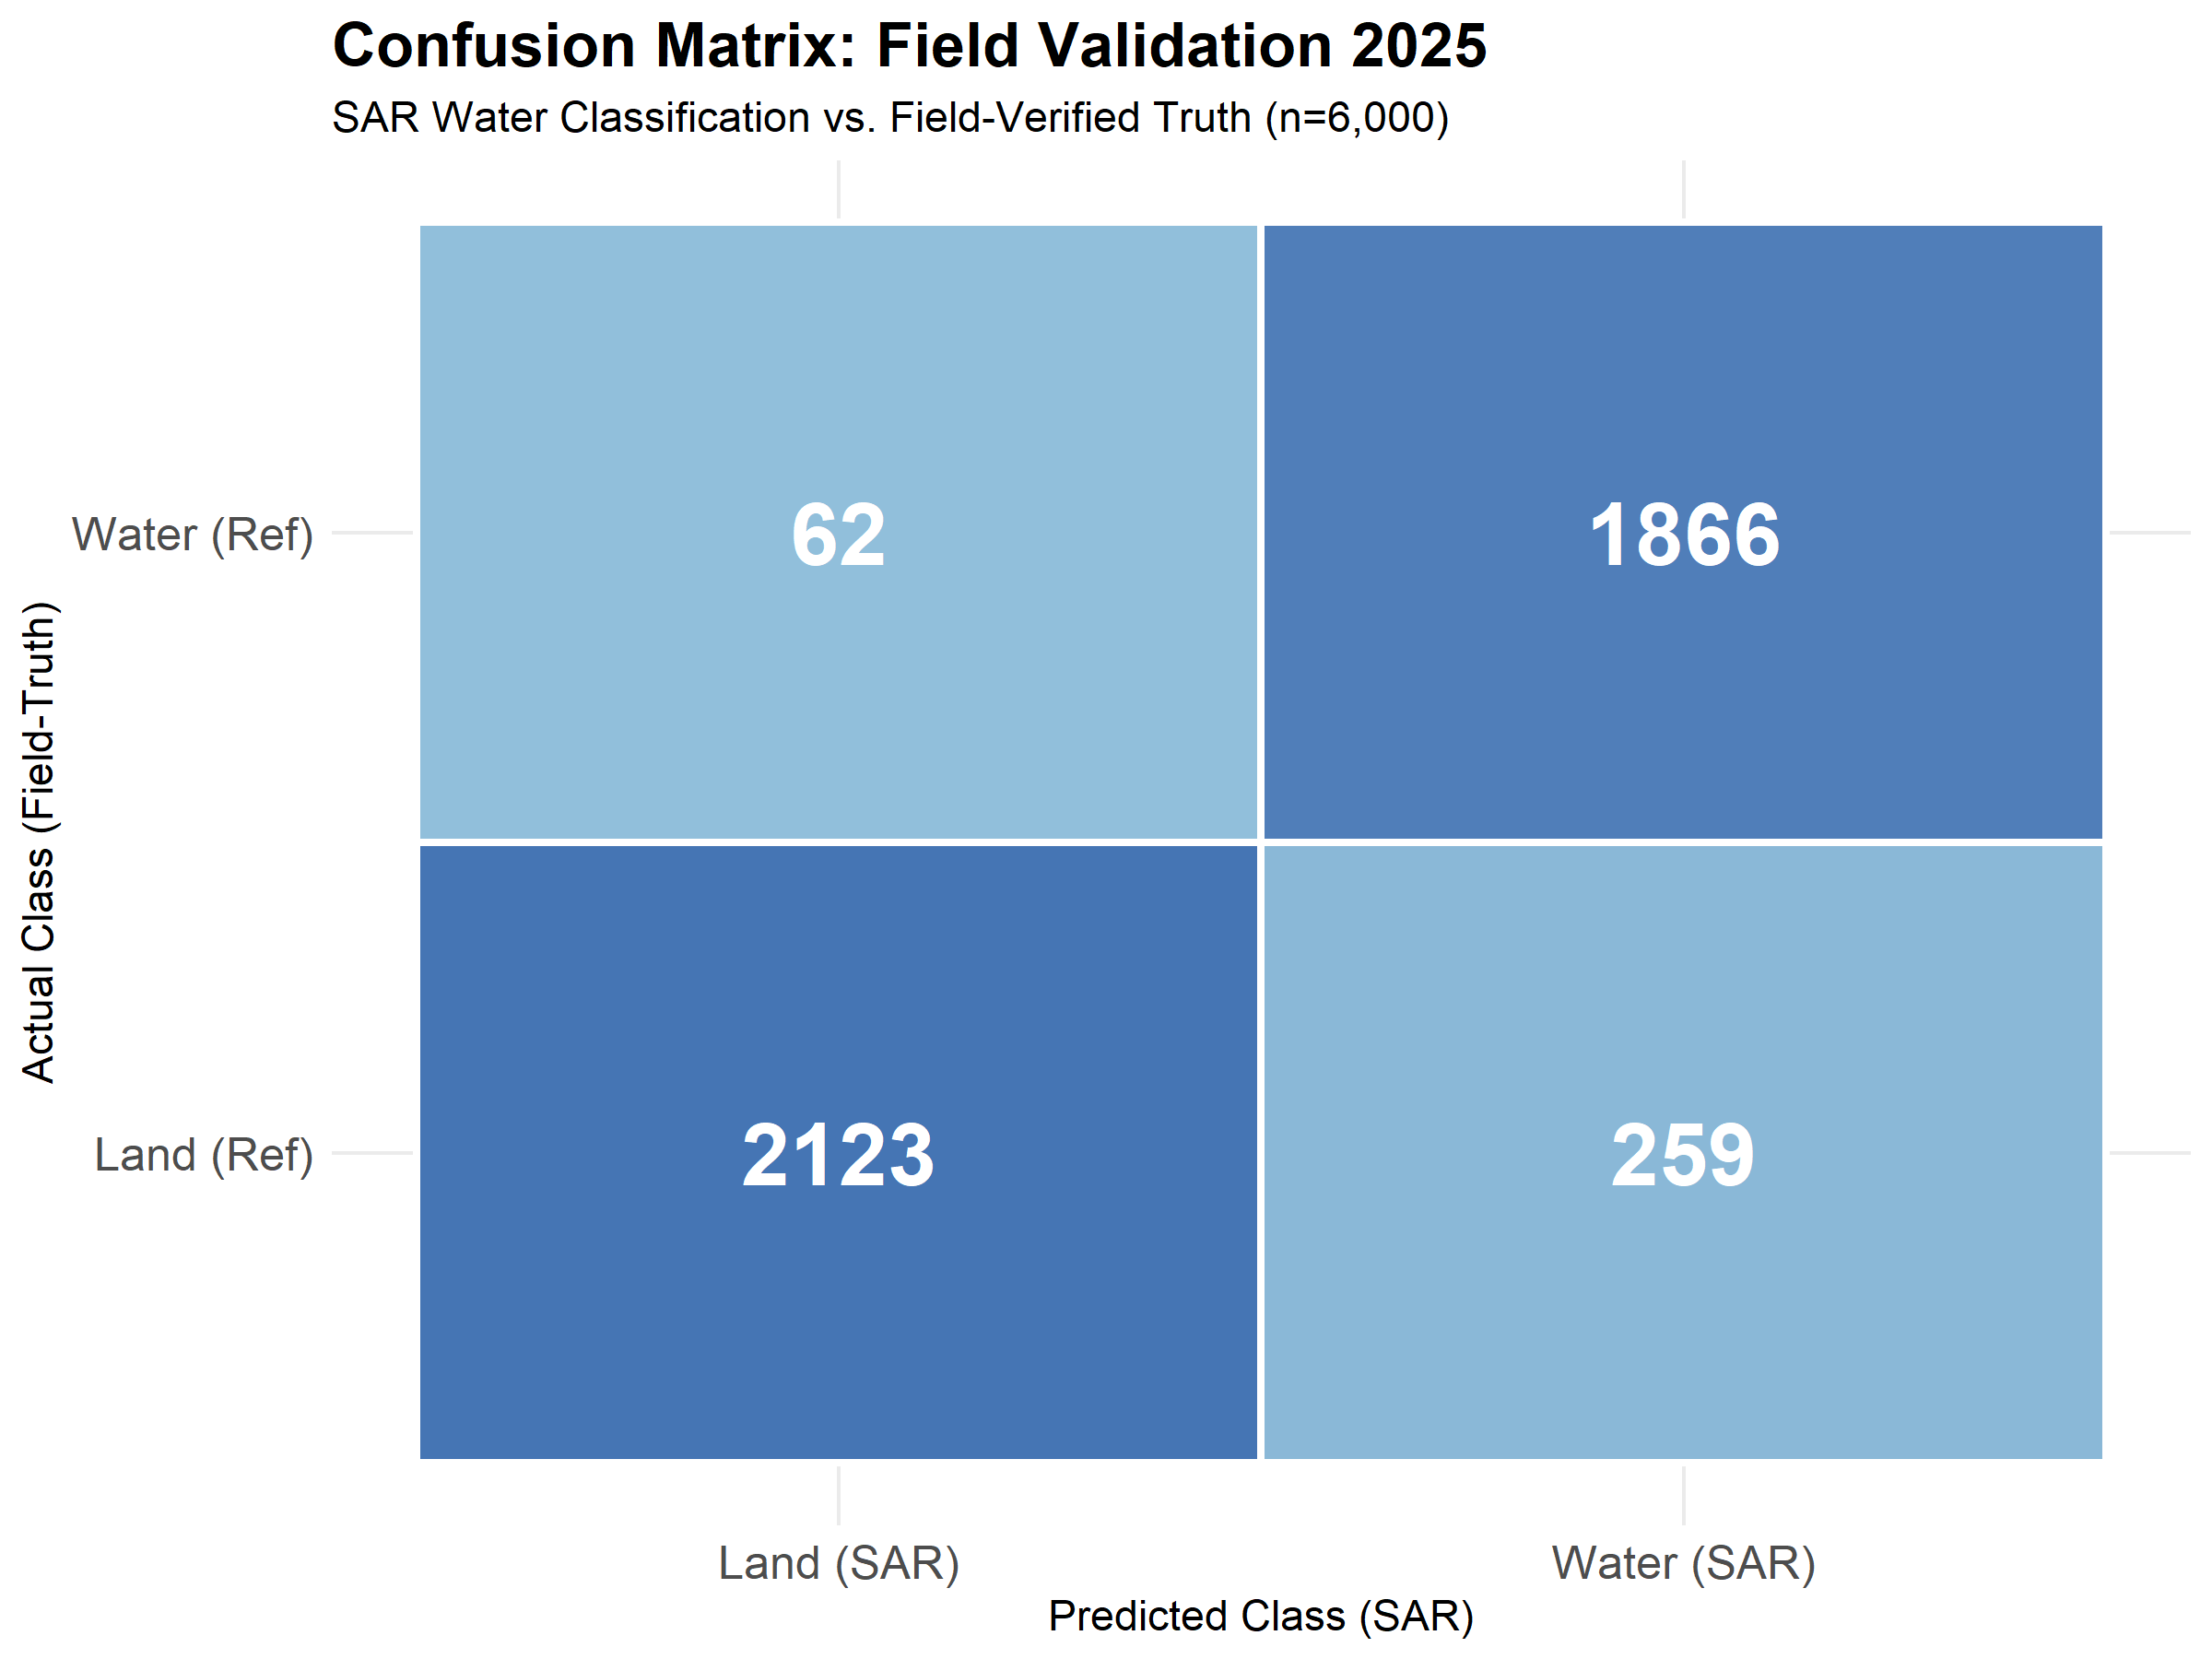
\includegraphics[width=0.7\textwidth]{figures/fig10_confusion_matrix_2025.png}
    \caption{\textbf{Supplementary Figure S10.} Confusion matrix for SAR-derived surface water classification against 6,000 field-verified reference points (2025). Note: the embedded subtitle in the figure file displays $n = 4{,}310$ from an earlier validation phase; this is a rendering artifact and should be disregarded.}
    \label{fig:s_cm}
\end{figure}

\begin{figure}[H]
    \centering
    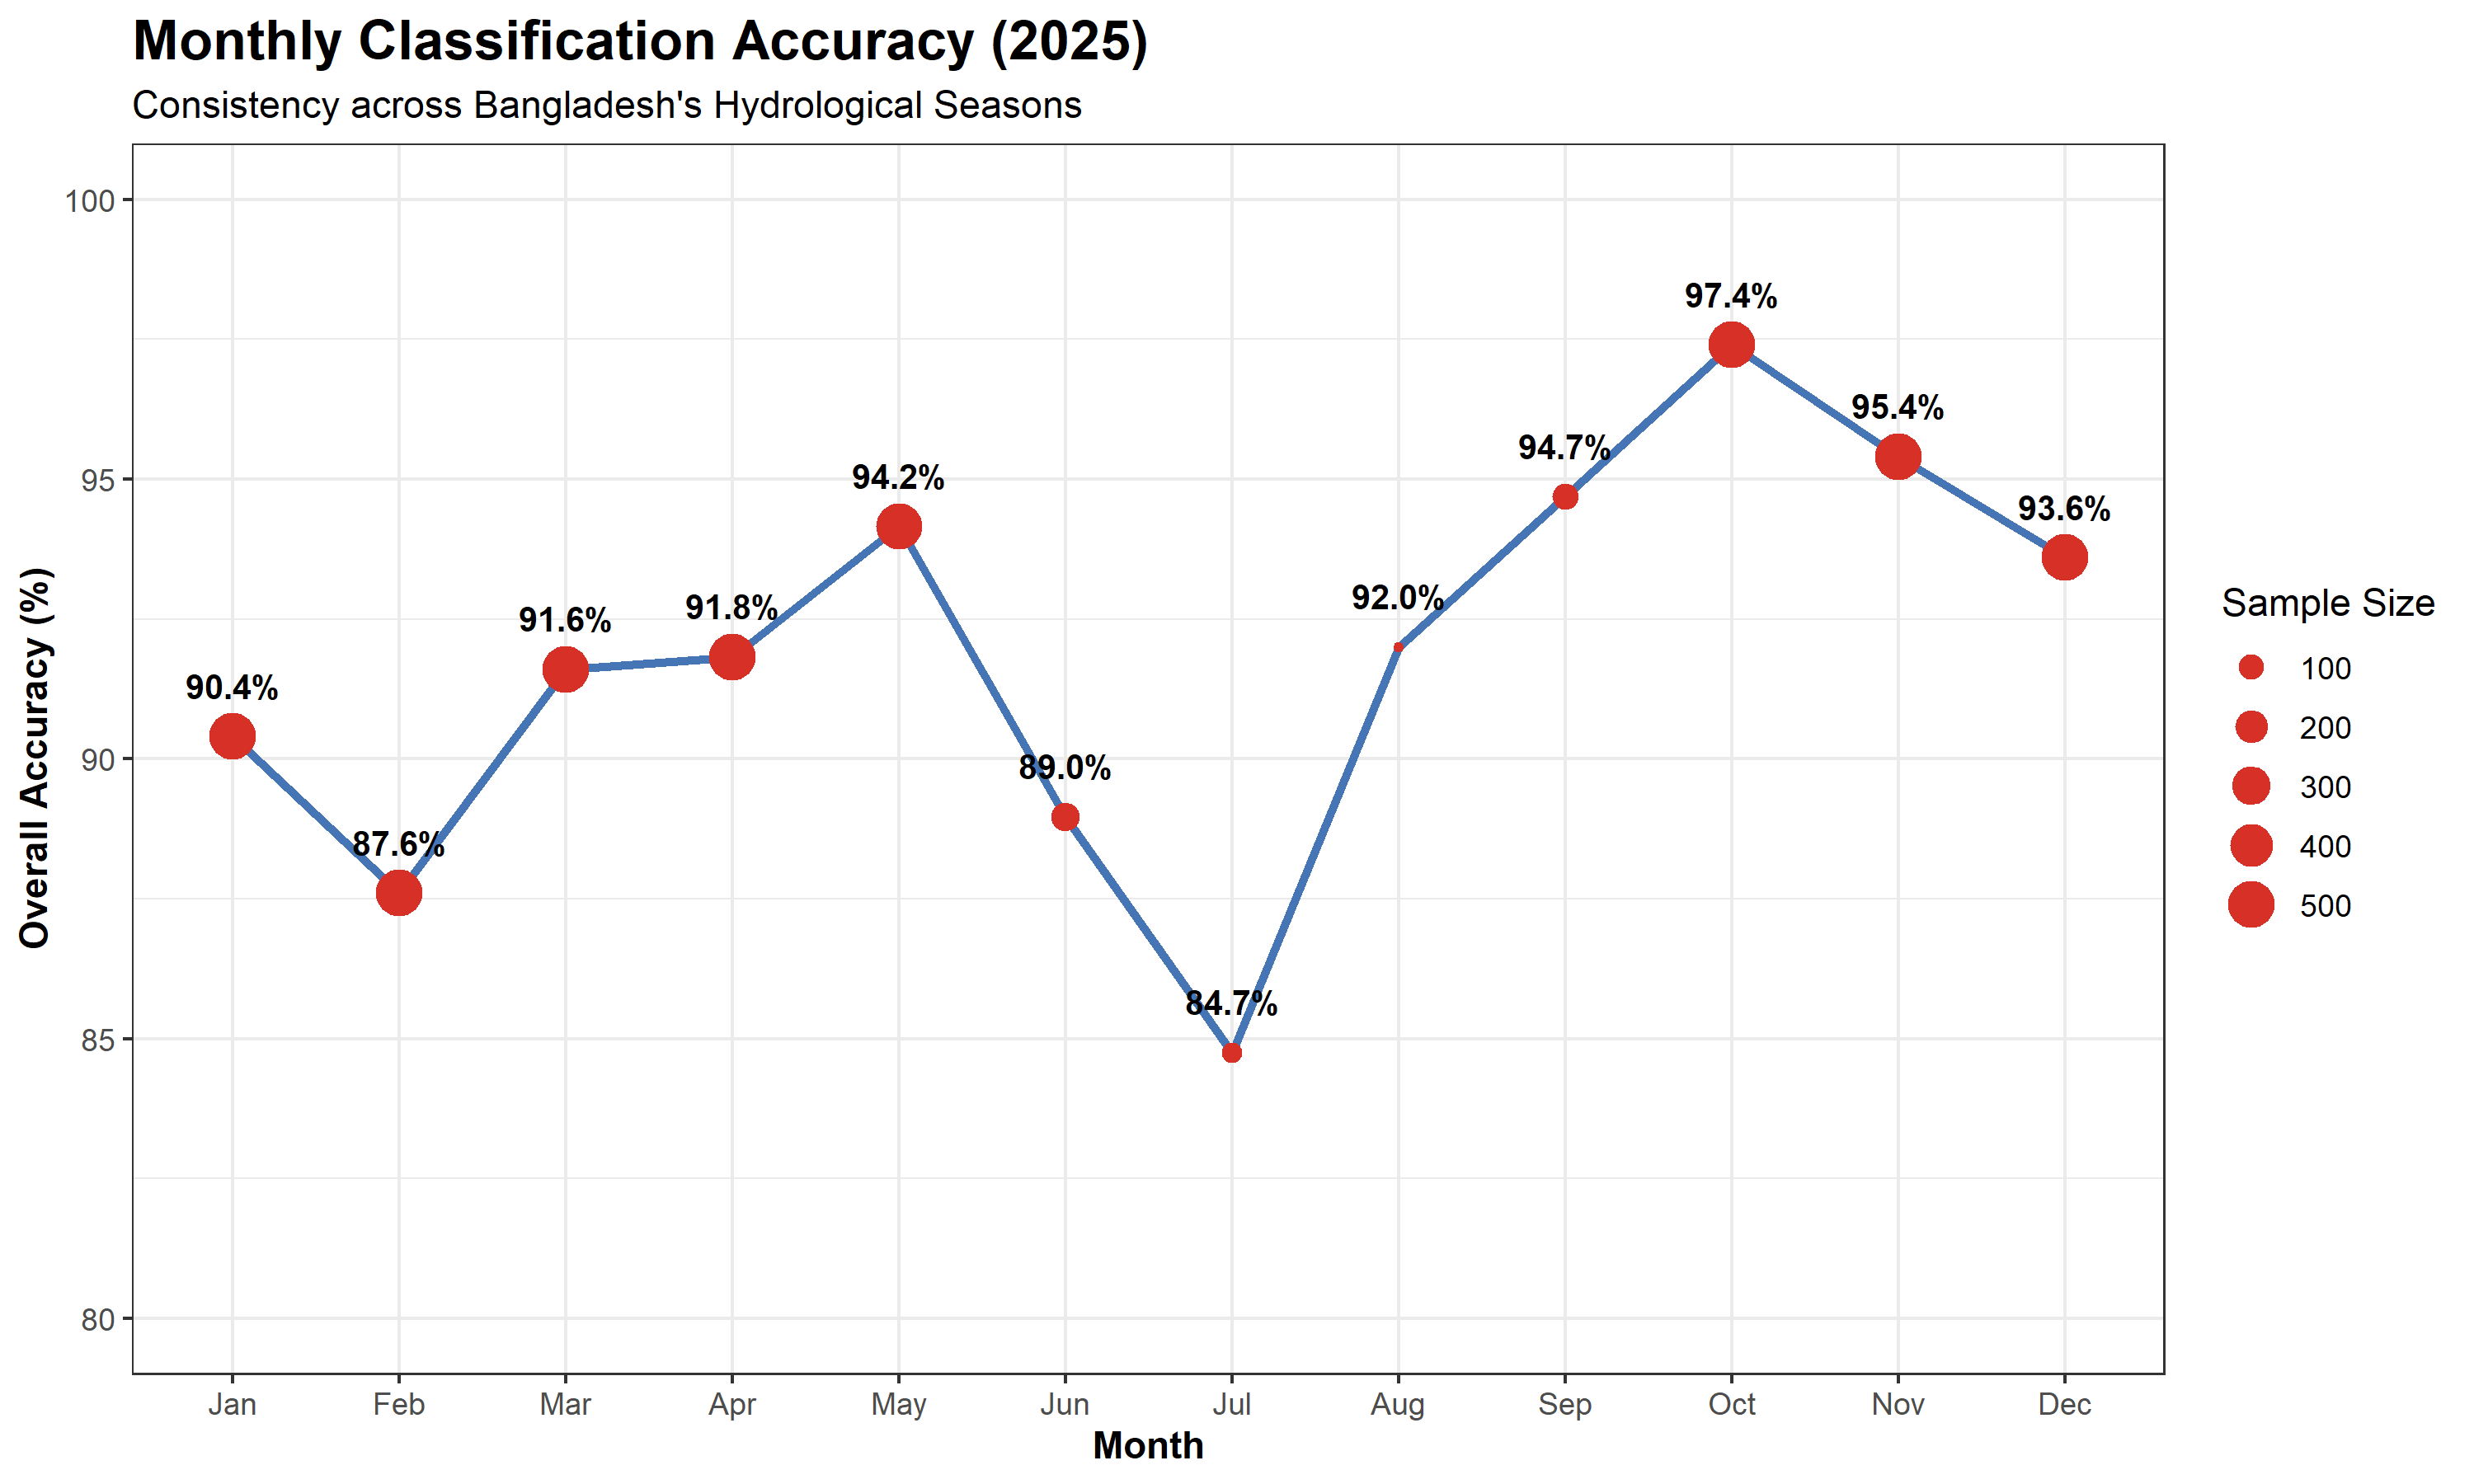
\includegraphics[width=0.9\textwidth]{figures/fig11_monthly_accuracy_2025.png}
    \caption{\textbf{Supplementary Figure S11.} Monthly overall accuracy (OA\%) of the SAR-based water monitoring framework for 2025.}
    \label{fig:s_monthly_acc}
\end{figure}


% Method comparison moved to main text (Figure 7)


% =========================
% Supplementary Figures S14-S20 - Regional Trend Plots
% =========================
\begin{figure}[H]
    \centering
    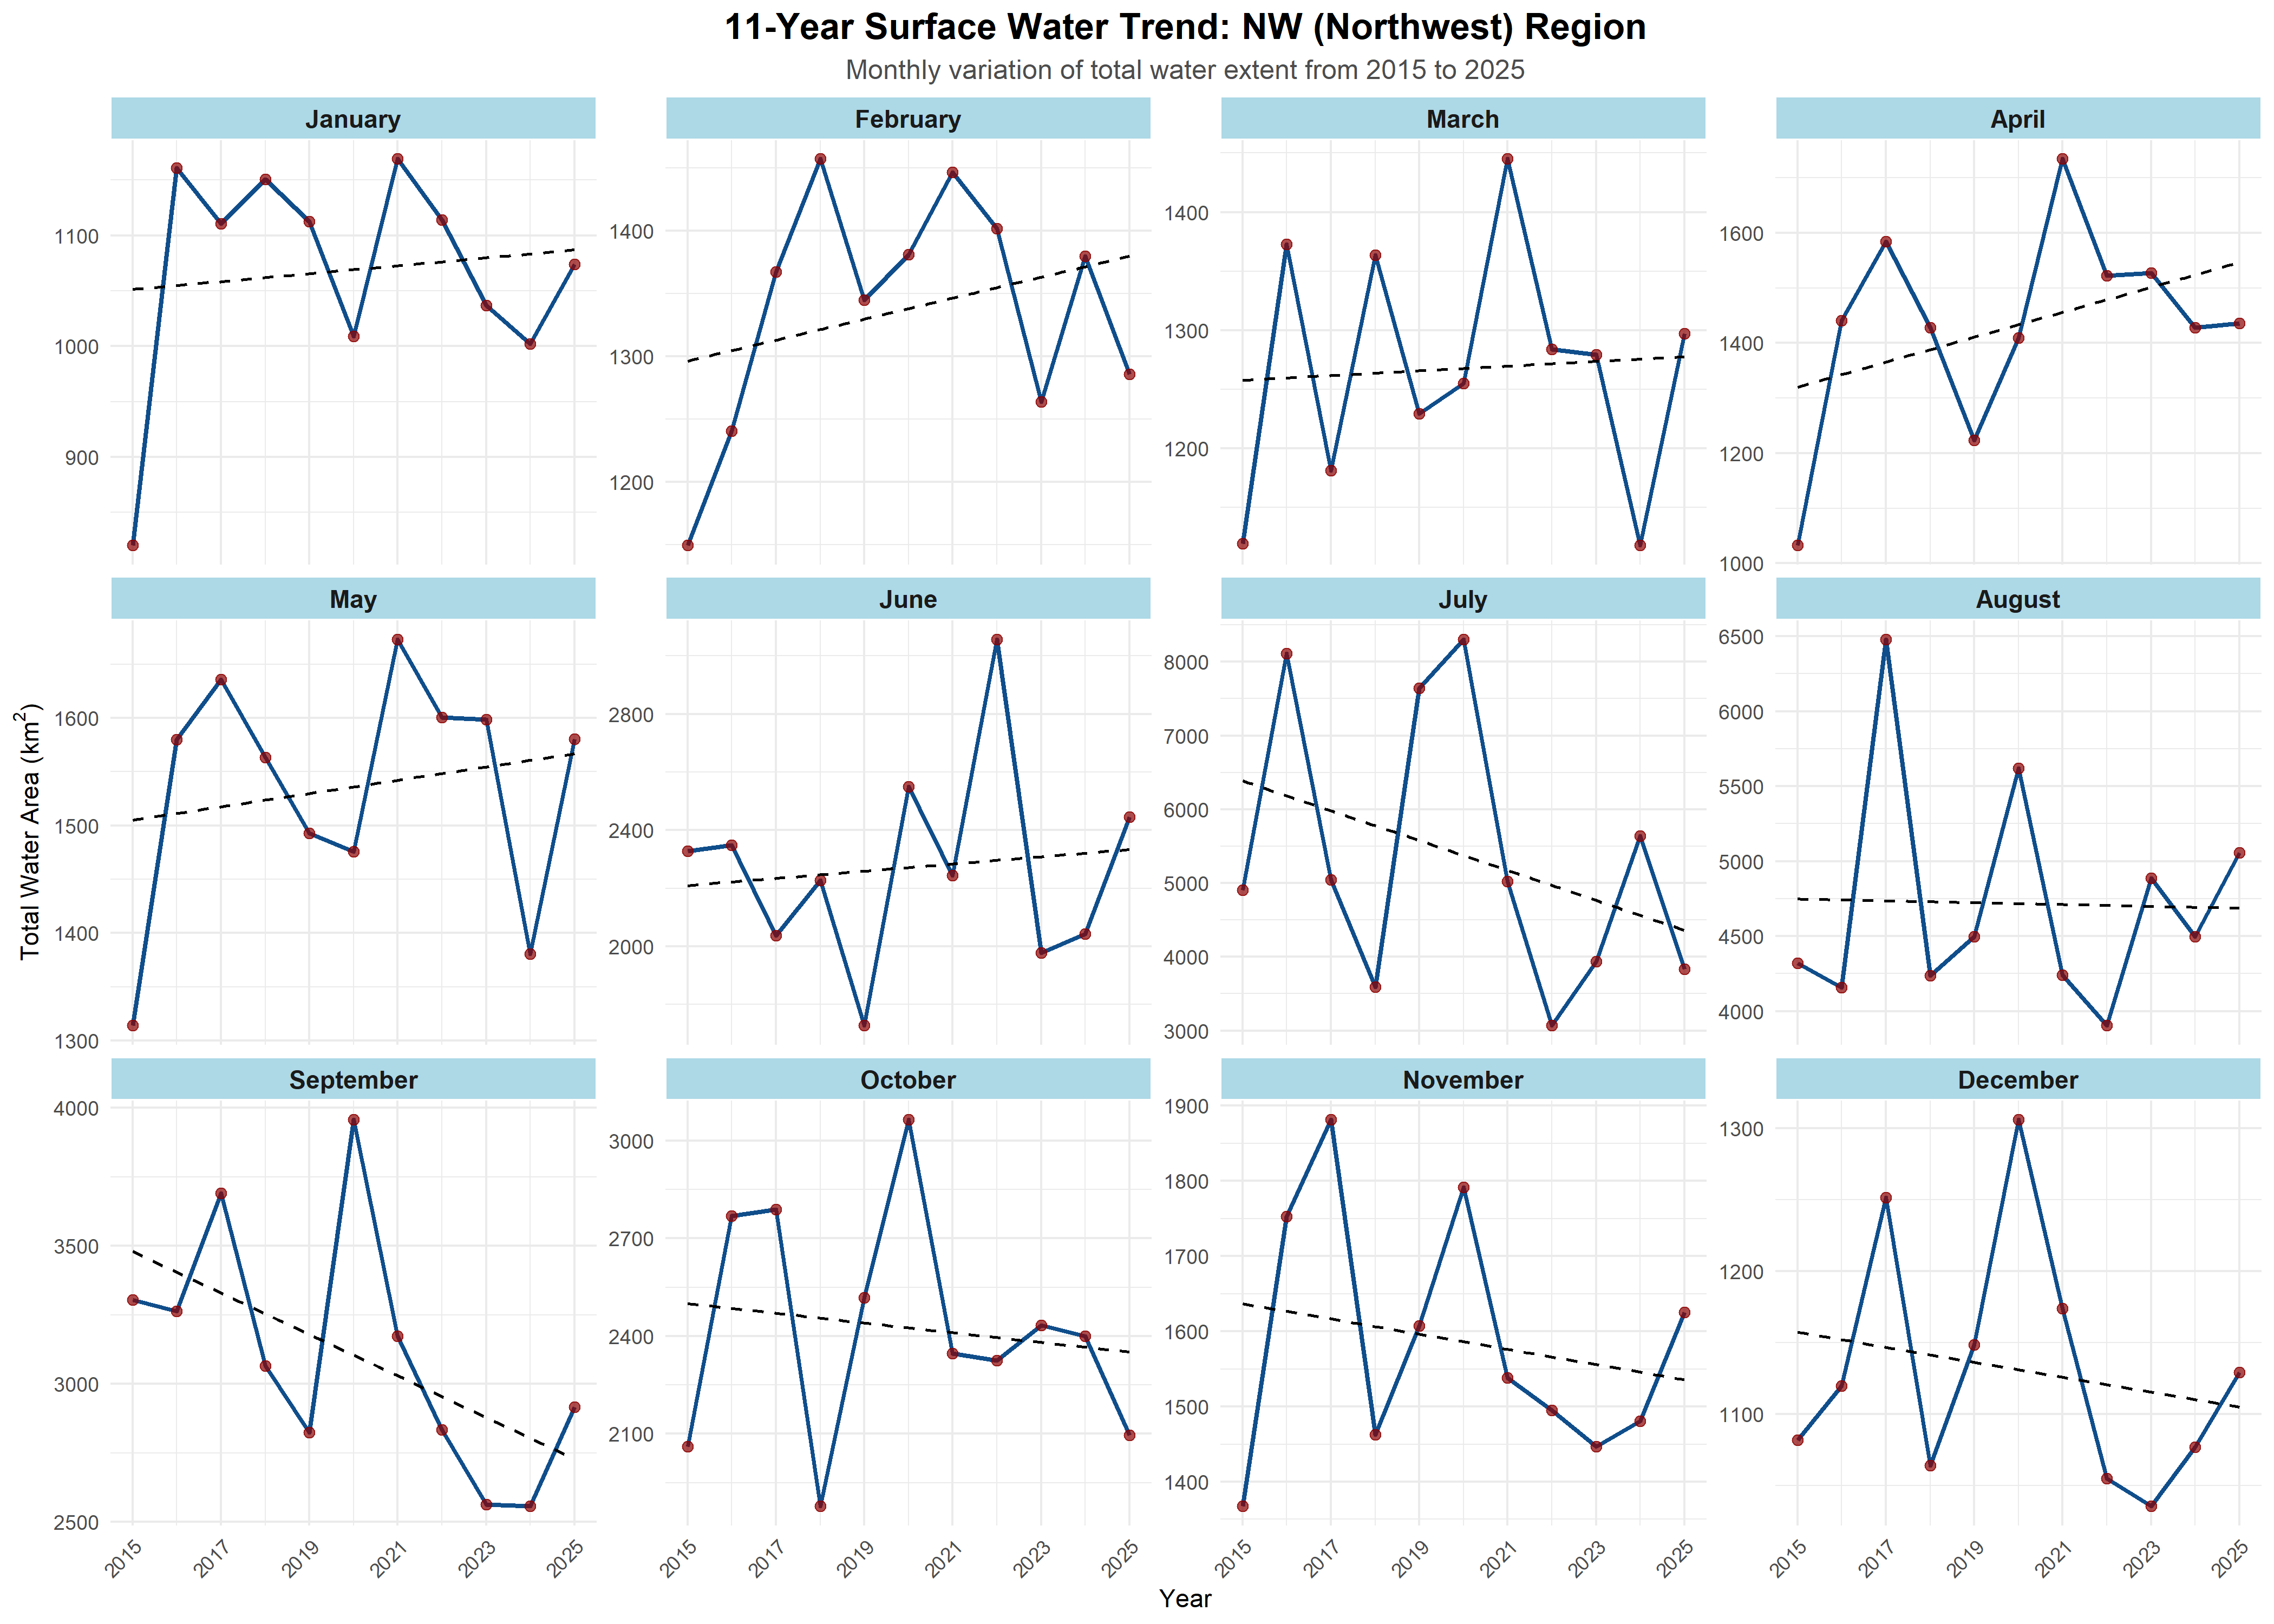
\includegraphics[width=0.95\textwidth]{figures/regional_trends/Plot_NW__Northwest_.png}
    \caption*{\textbf{Supplementary Figure S12.} 11-Year Surface Water Trend for the Northwest (NW) Region across all 12 months.}
    \label{fig:s_nw}
\end{figure}

\begin{figure}[H]
    \centering
    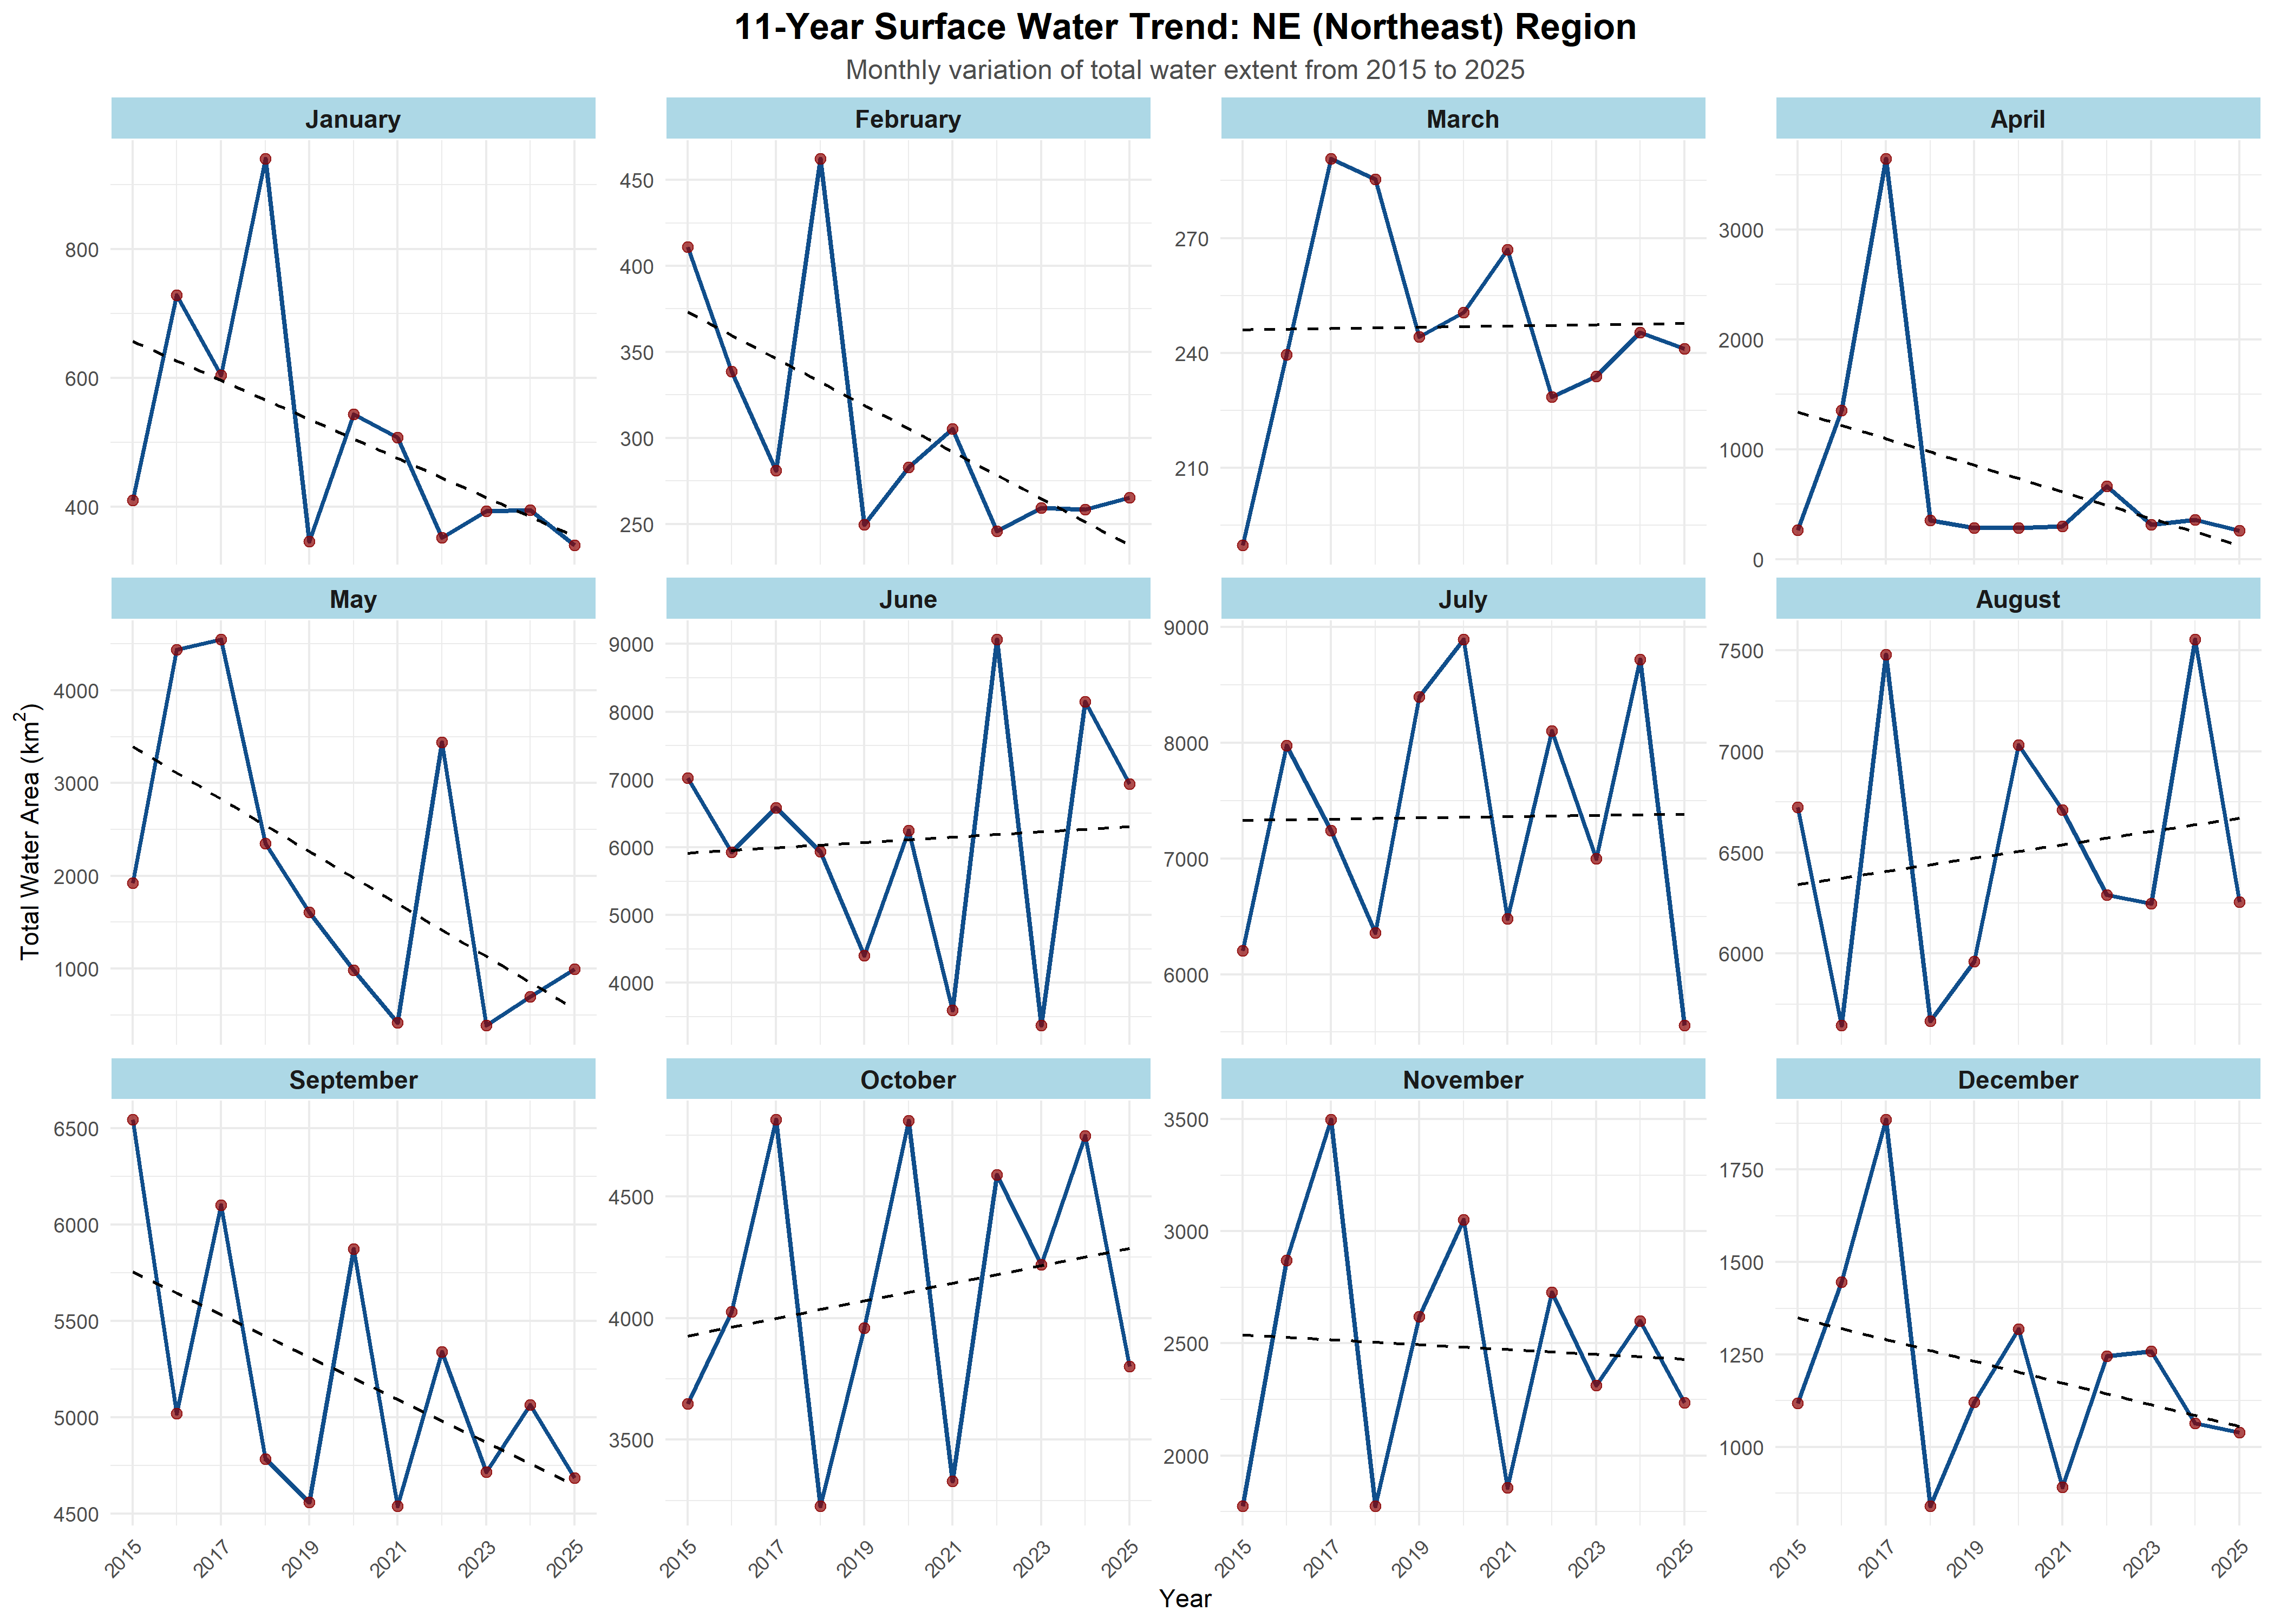
\includegraphics[width=0.95\textwidth]{figures/regional_trends/Plot_NE__Northeast_.png}
    \caption*{\textbf{Supplementary Figure S13.} 11-Year Surface Water Trend for the Northeast (NE) Region across all 12 months.}
    \label{fig:s_ne}
\end{figure}

\begin{figure}[H]
    \centering
    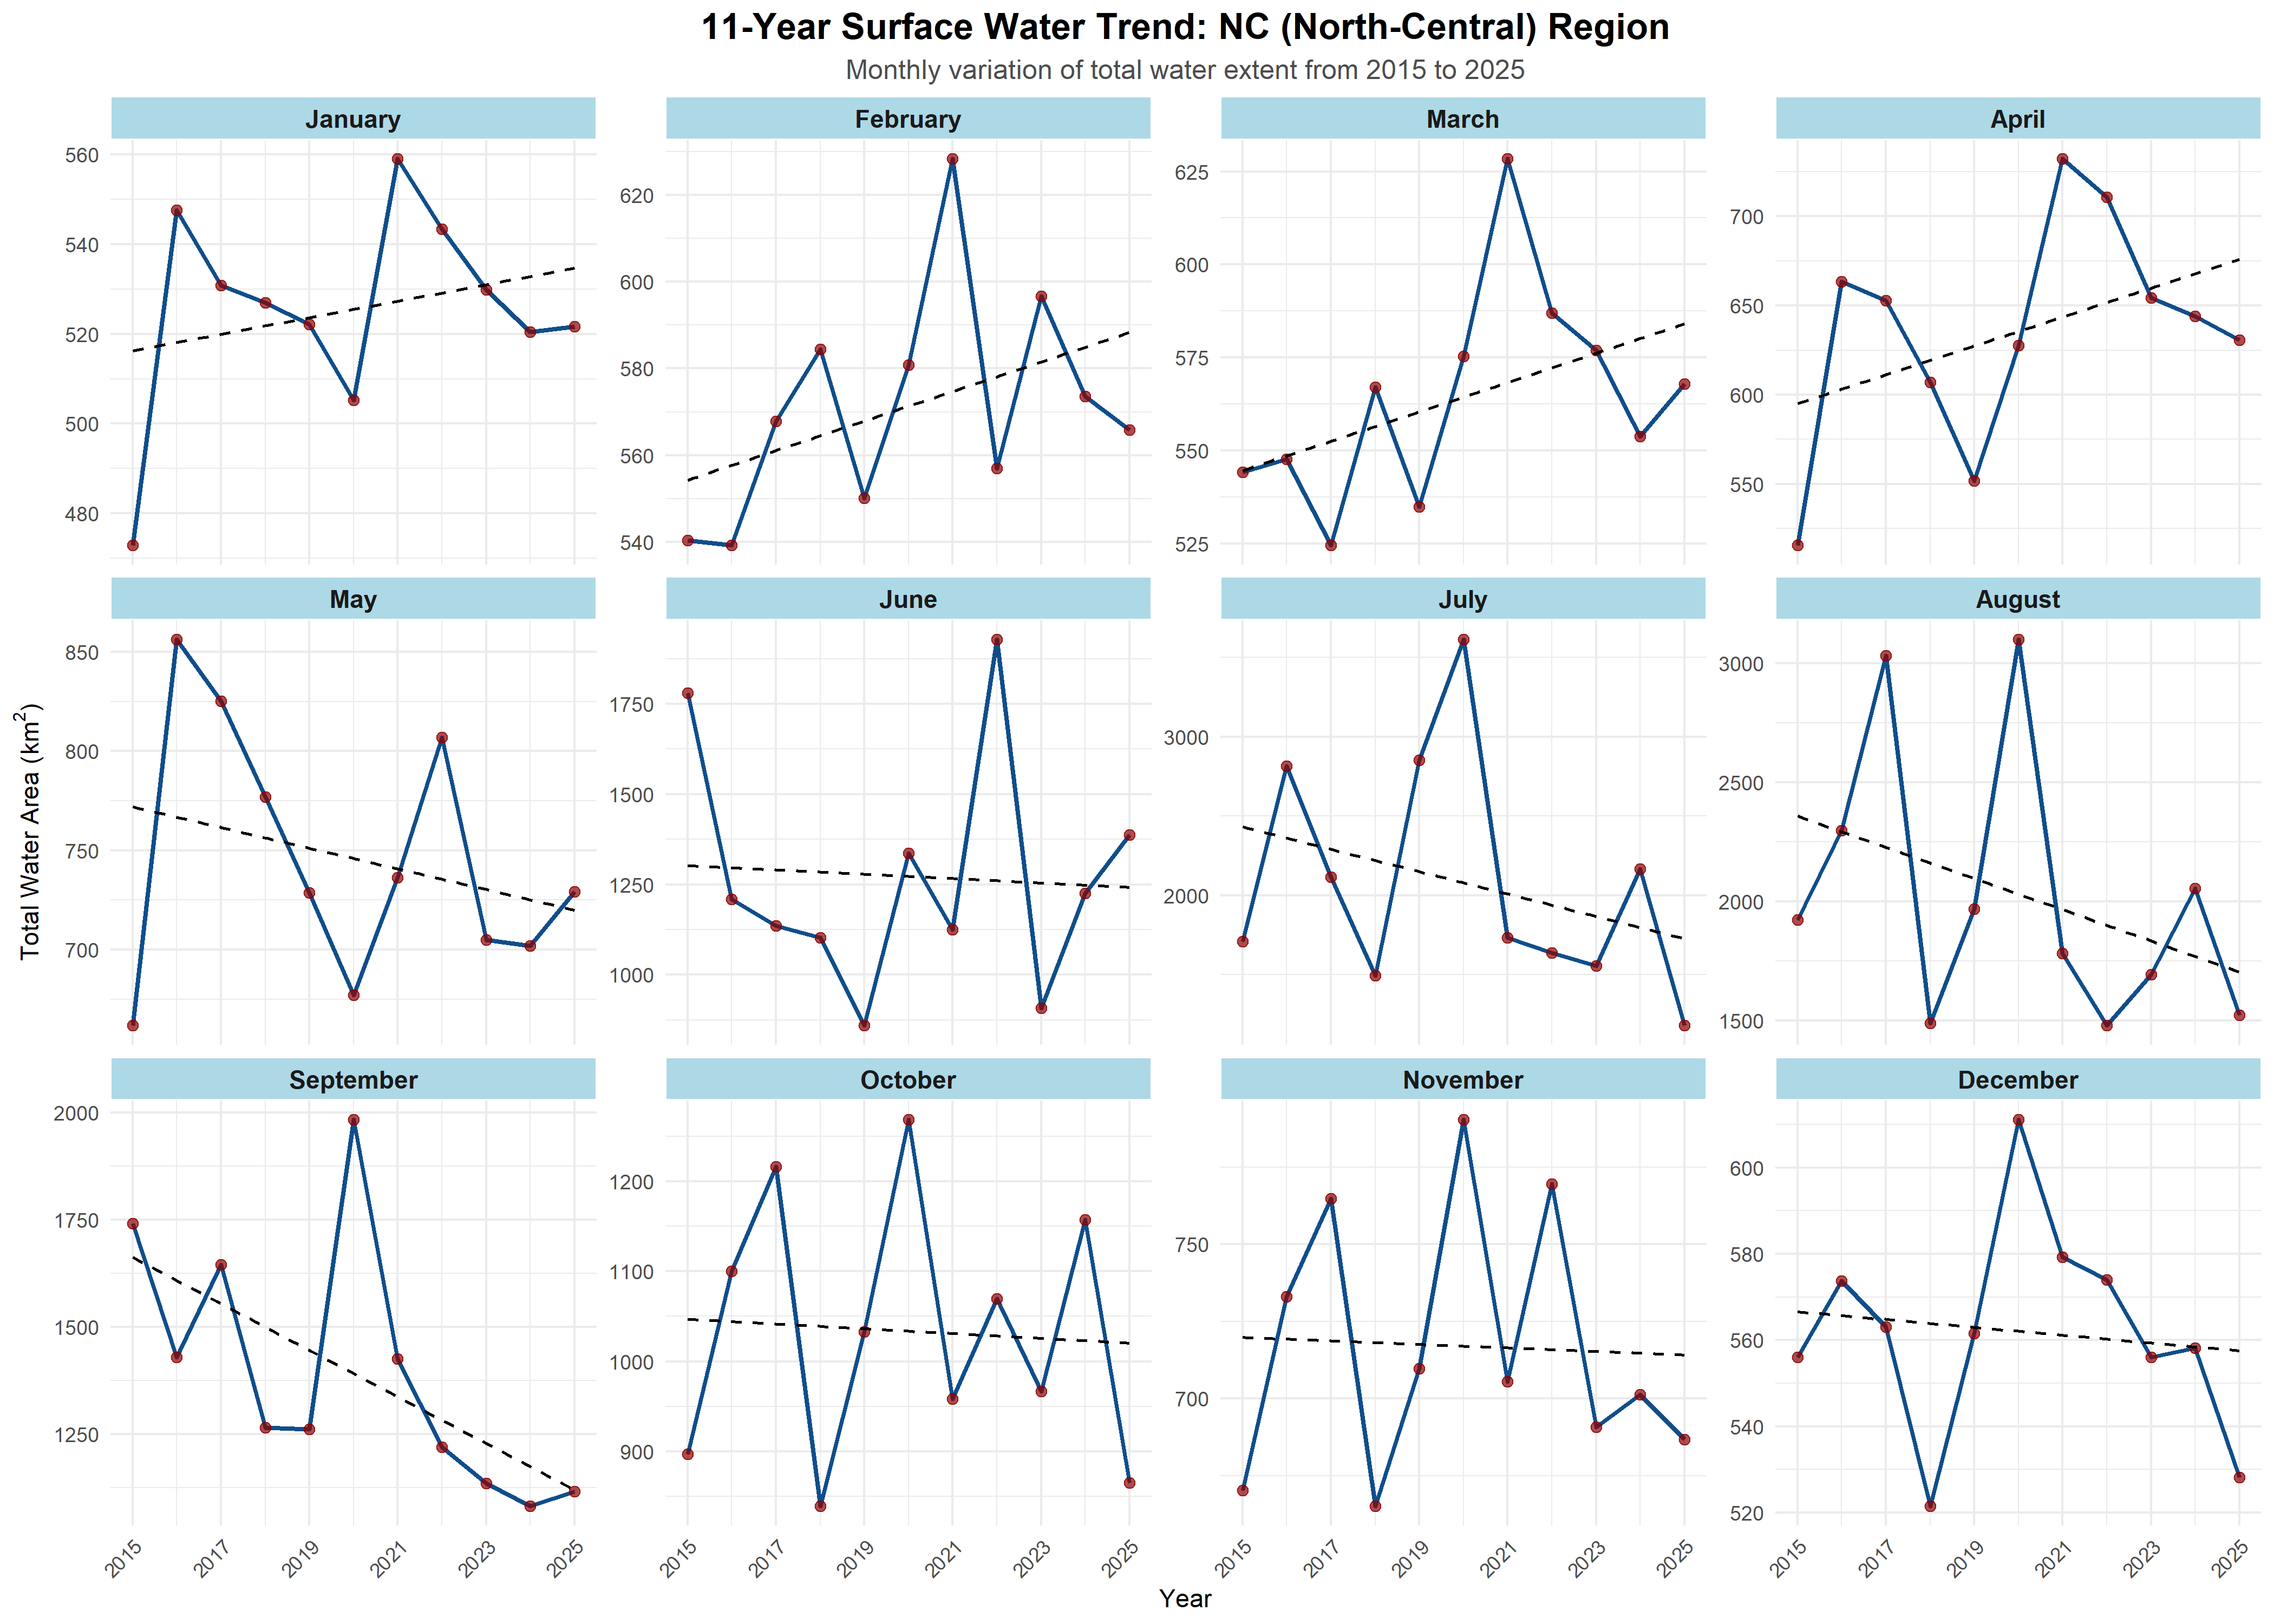
\includegraphics[width=0.95\textwidth]{figures/regional_trends/Plot_NC__North_Central_.png}
    \caption*{\textbf{Supplementary Figure S14.} 11-Year Surface Water Trend for the North-Central (NC) Region across all 12 months.}
    \label{fig:s_nc}
\end{figure}

\begin{figure}[H]
    \centering
    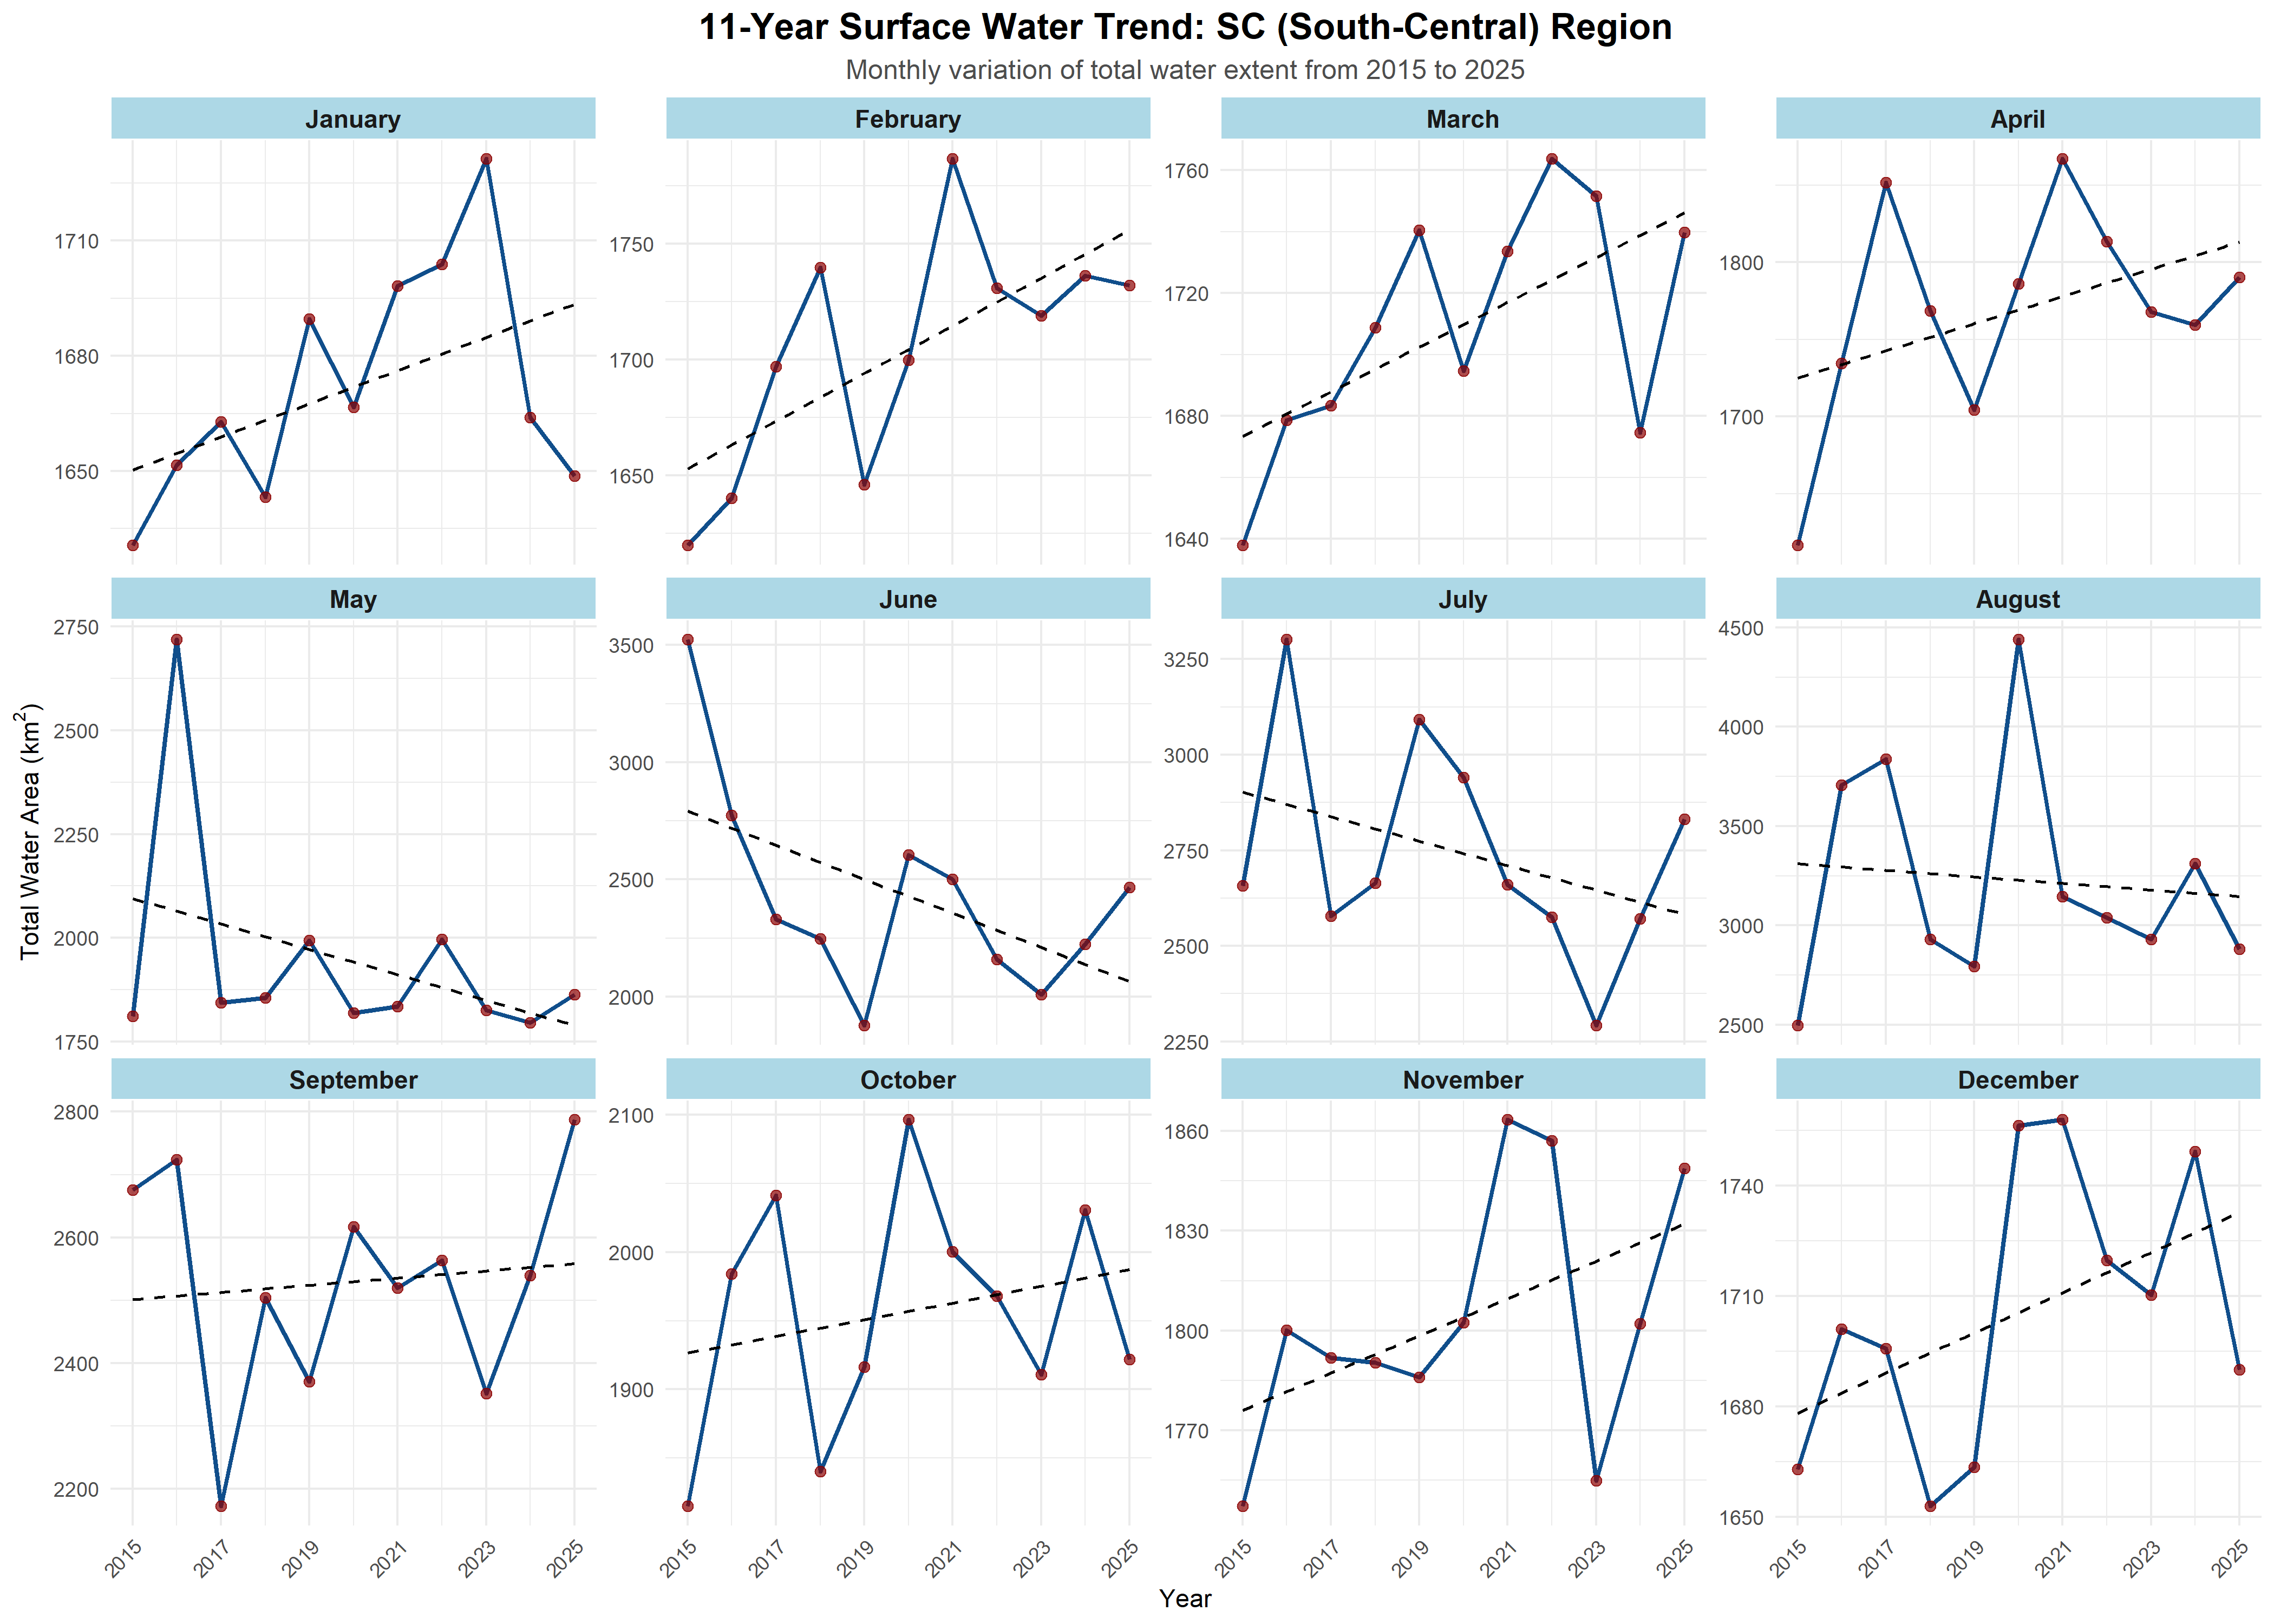
\includegraphics[width=0.95\textwidth]{figures/regional_trends/Plot_SC__South_Central_.png}
    \caption*{\textbf{Supplementary Figure S15.} 11-Year Surface Water Trend for the South-Central (SC) Region across all 12 months.}
    \label{fig:s_sc}
\end{figure}

\begin{figure}[H]
    \centering
    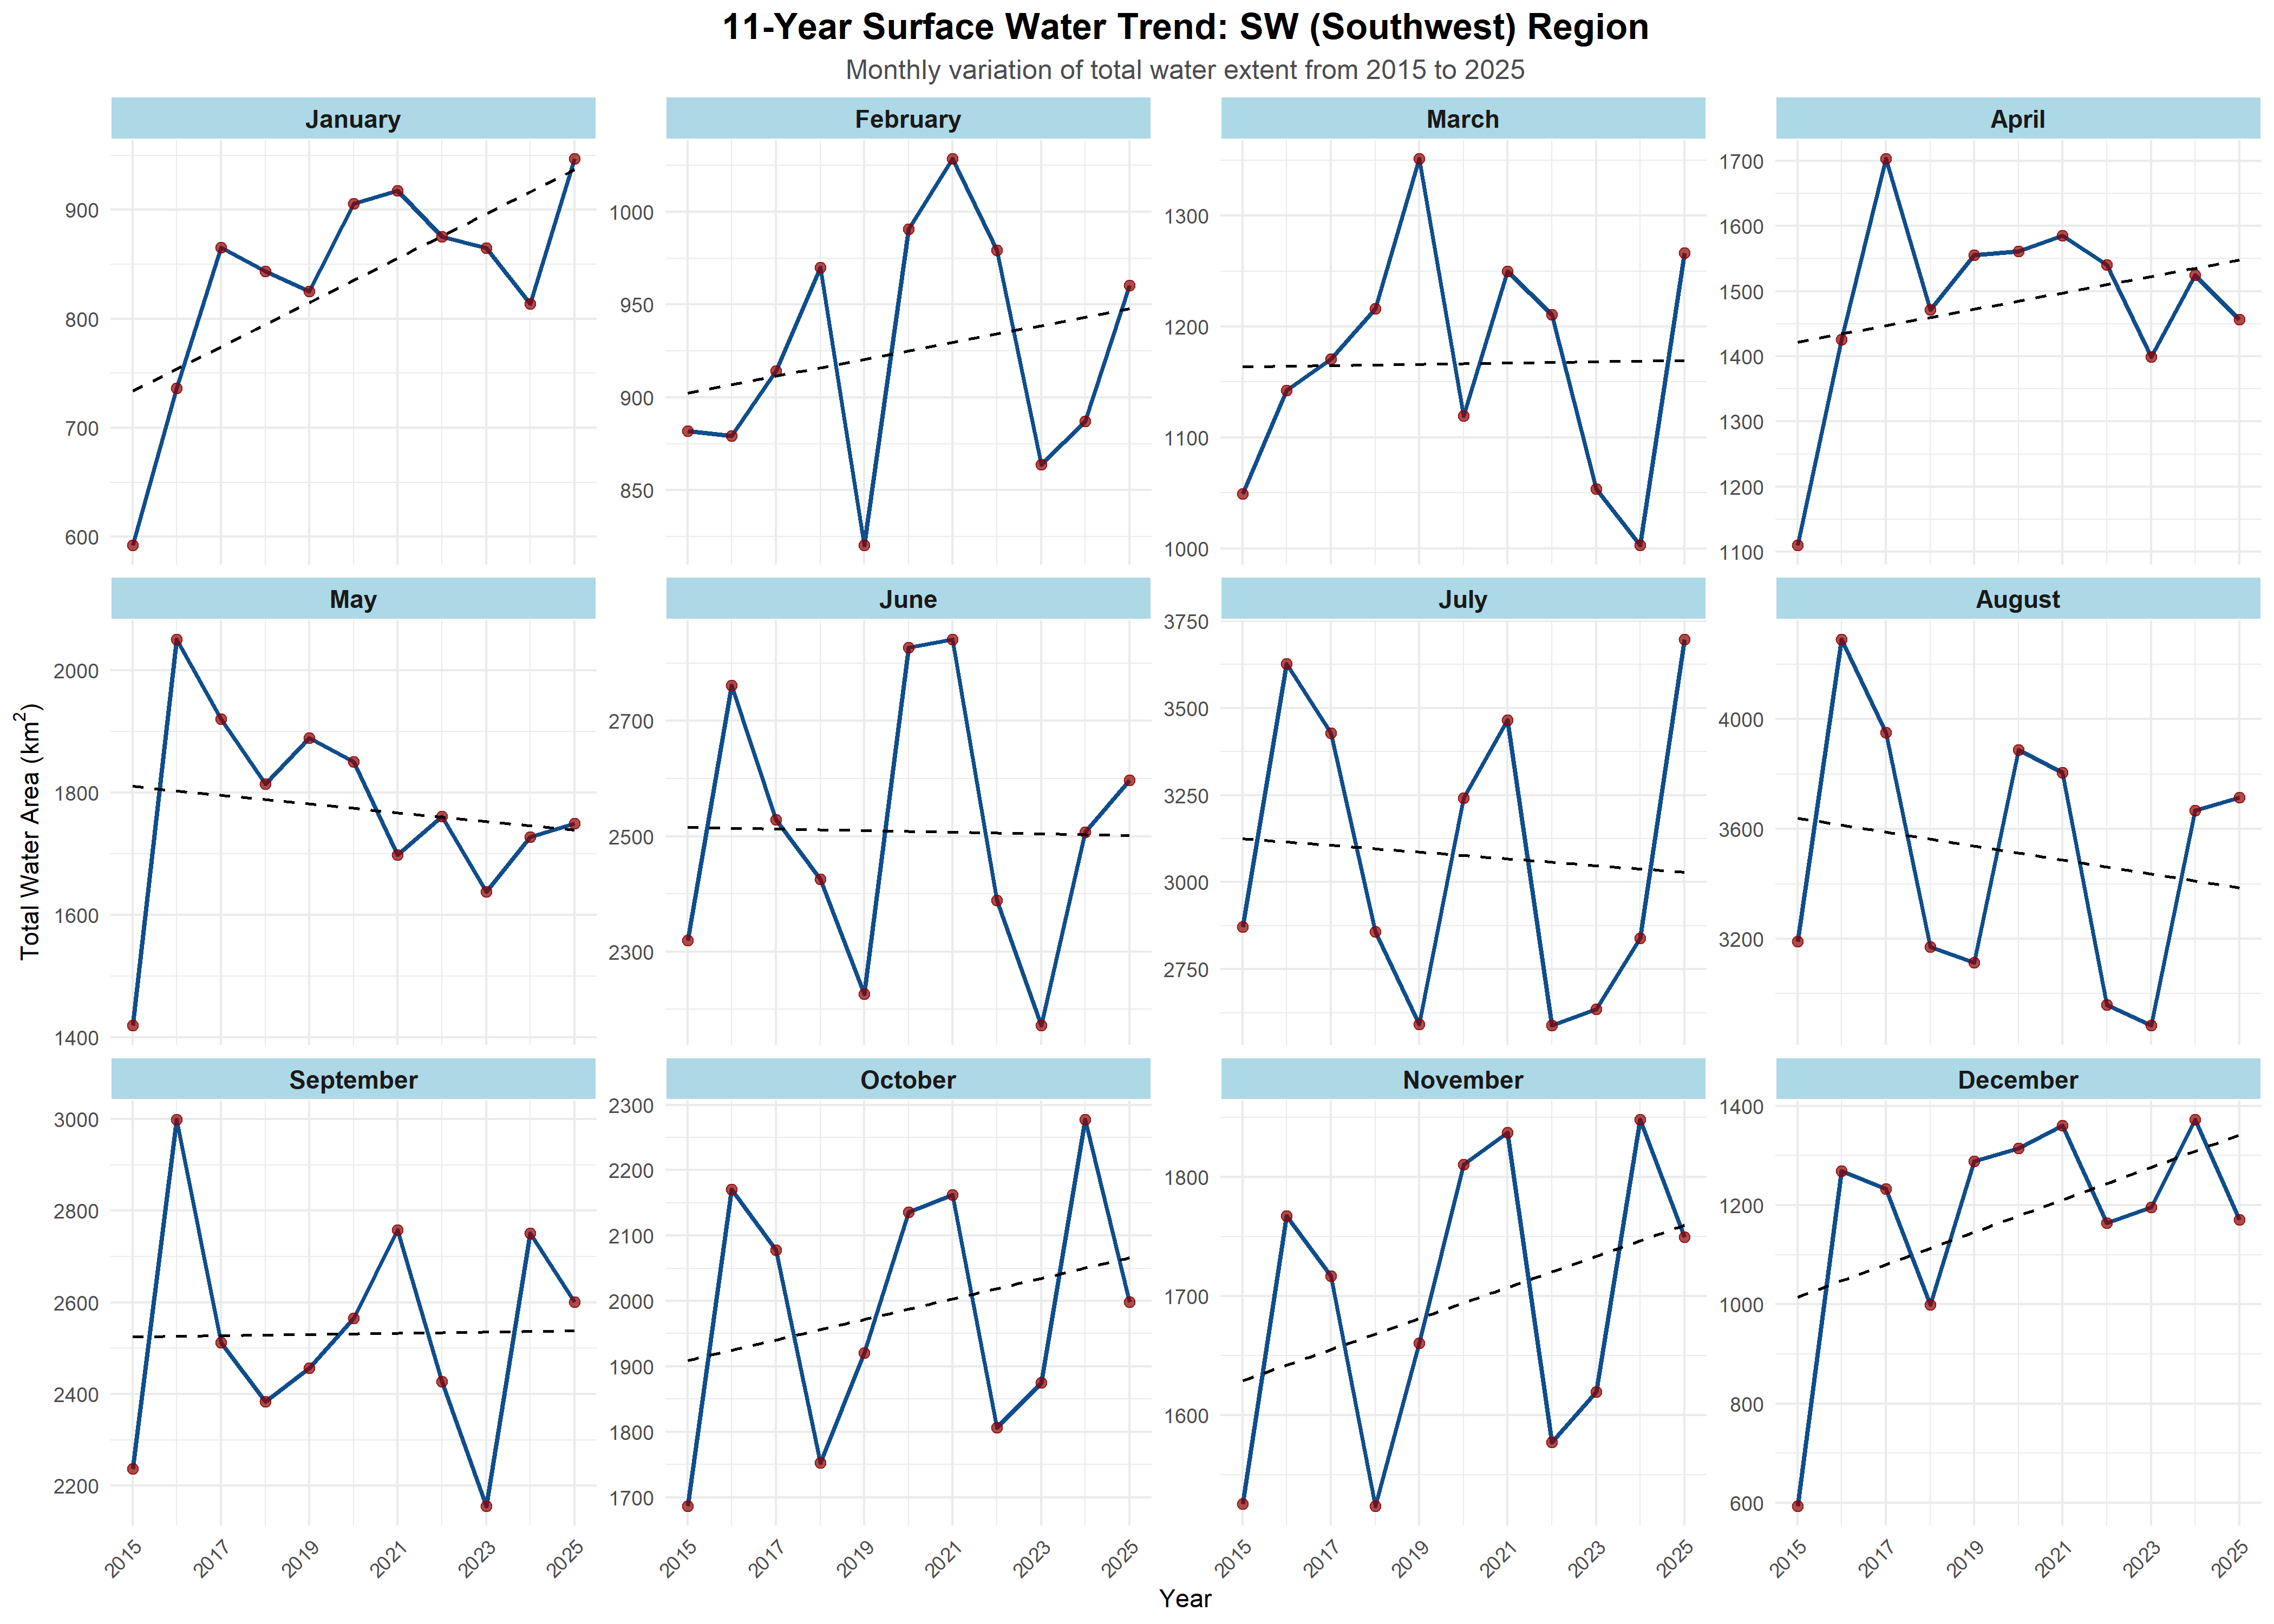
\includegraphics[width=0.95\textwidth]{figures/regional_trends/Plot_SW__Southwest_.png}
    \caption*{\textbf{Supplementary Figure S16.} 11-Year Surface Water Trend for the Southwest (SW) Region across all 12 months.}
    \label{fig:s_sw}
\end{figure}

\begin{figure}[H]
    \centering
    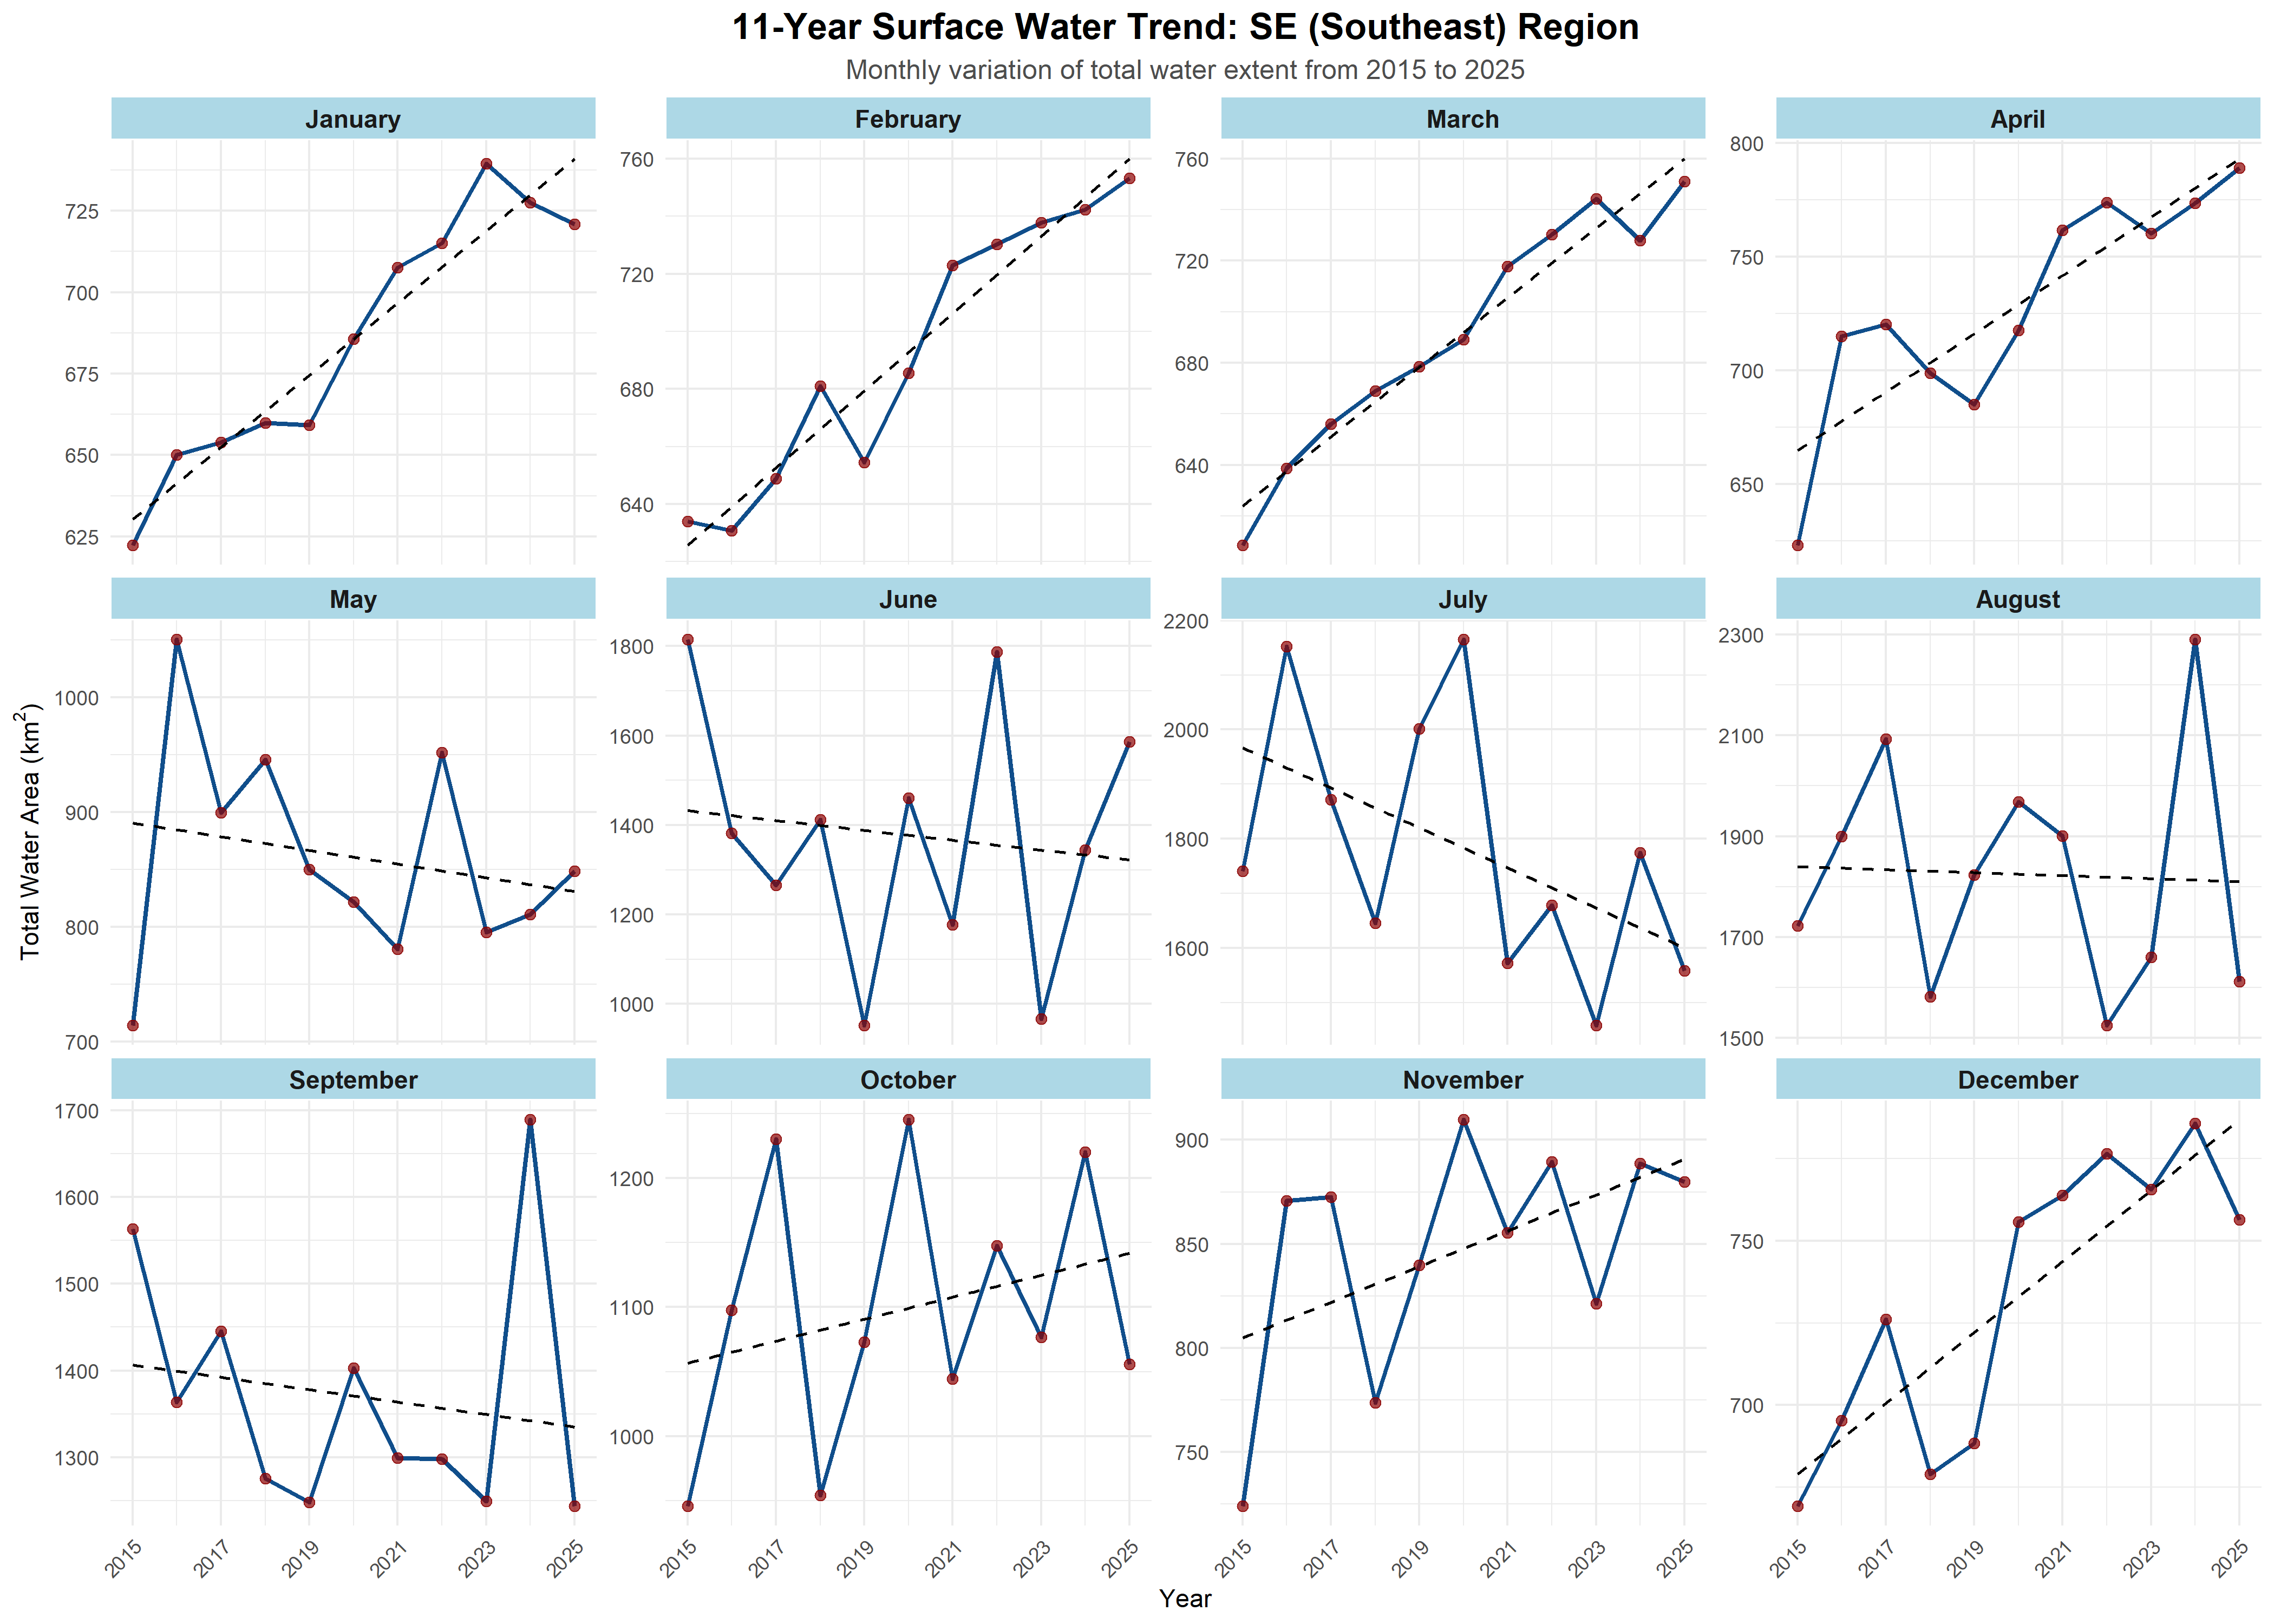
\includegraphics[width=0.95\textwidth]{figures/regional_trends/Plot_SE__Southeast_.png}
    \caption*{\textbf{Supplementary Figure S17.} 11-Year Surface Water Trend for the Southeast (SE) Region across all 12 months.}
    \label{fig:s_se}
\end{figure}

\begin{figure}[H]
    \centering
    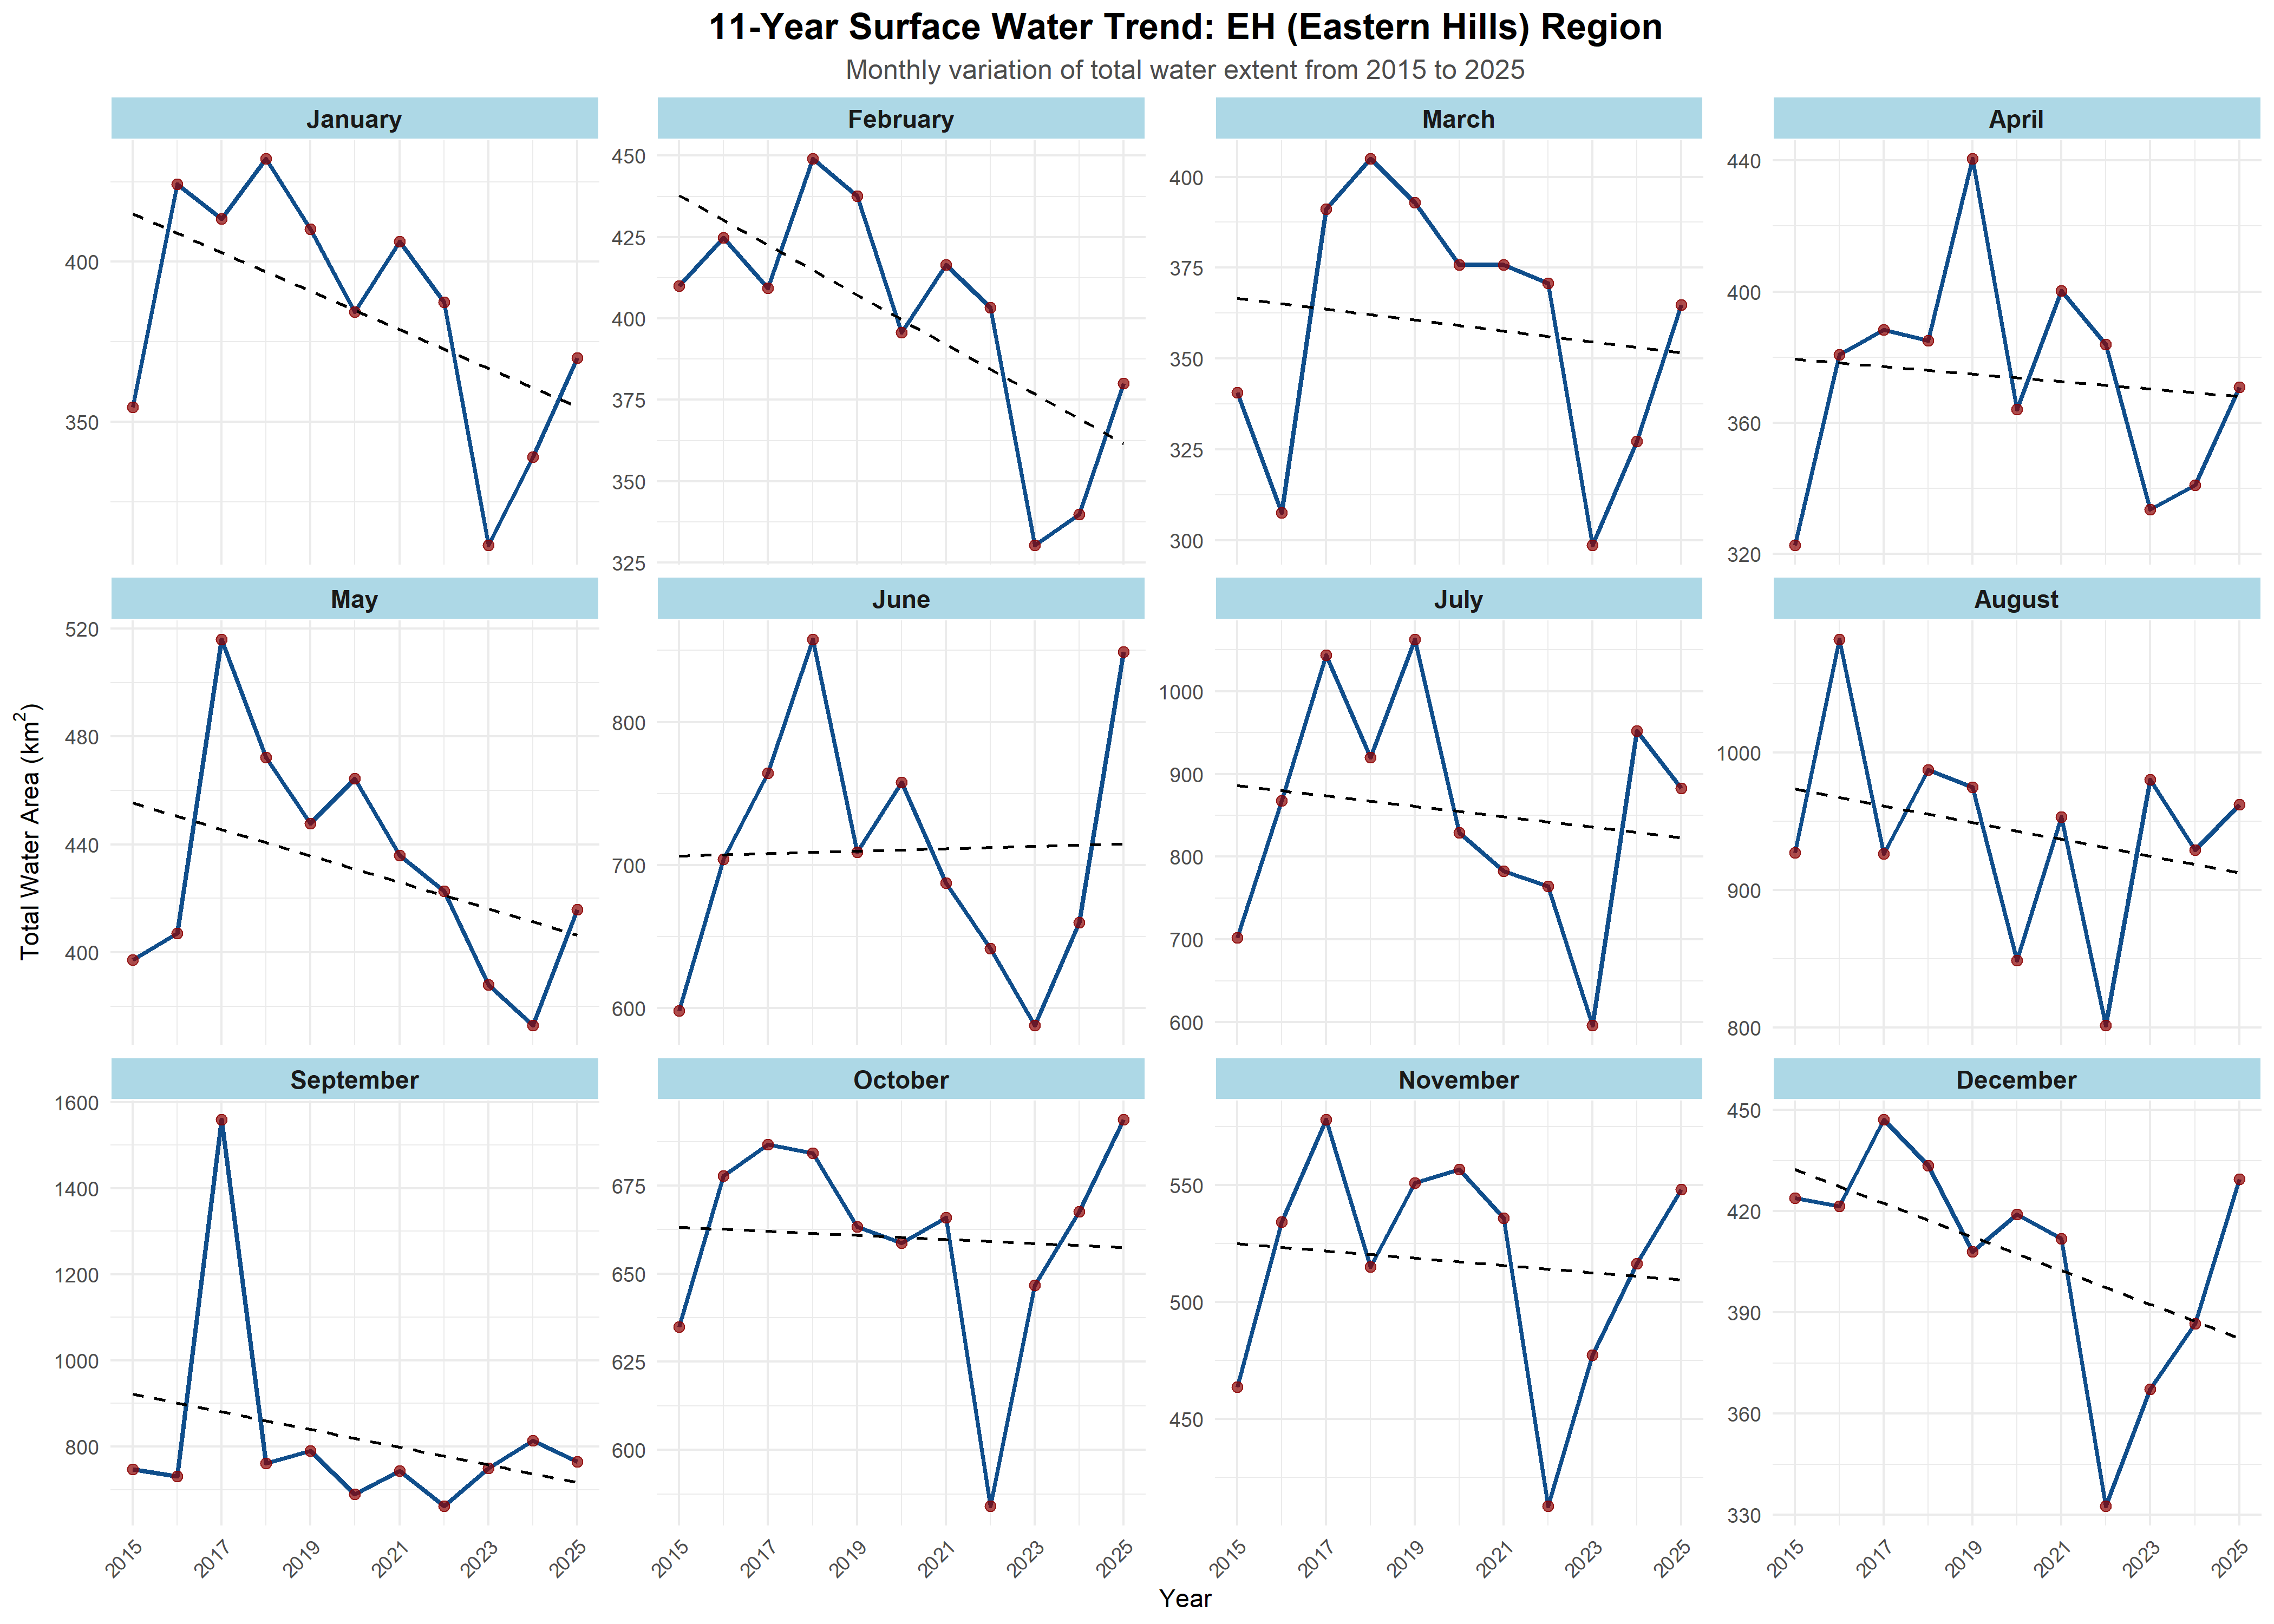
\includegraphics[width=0.95\textwidth]{figures/regional_trends/Plot_EH__Eastern_Hills_.png}
    \caption*{\textbf{Supplementary Figure S18.} 11-Year Surface Water Trend for the Eastern Hills (EH) Region across all 12 months.}
    \label{fig:s_eh}
\end{figure}

\end{document}
